\section{Beamline geometry}

\subsection{The view from above}

If one were hovering above the beamline instrumentation with their head in the direction of the beam direction, then the forward direction is positive $z$, to the left is positive $x$, and the positive $y$ direction is upwards toward the sky. See diagram in Figure~\ref{fig_overview}. The coordinates of some main components are given in Figure~\ref{fig_coords}. Figure~\ref{fig_traj} shows an example trajectory of a particle through the beamline components.
\begin{figure}[h]	  
 \centering 
        	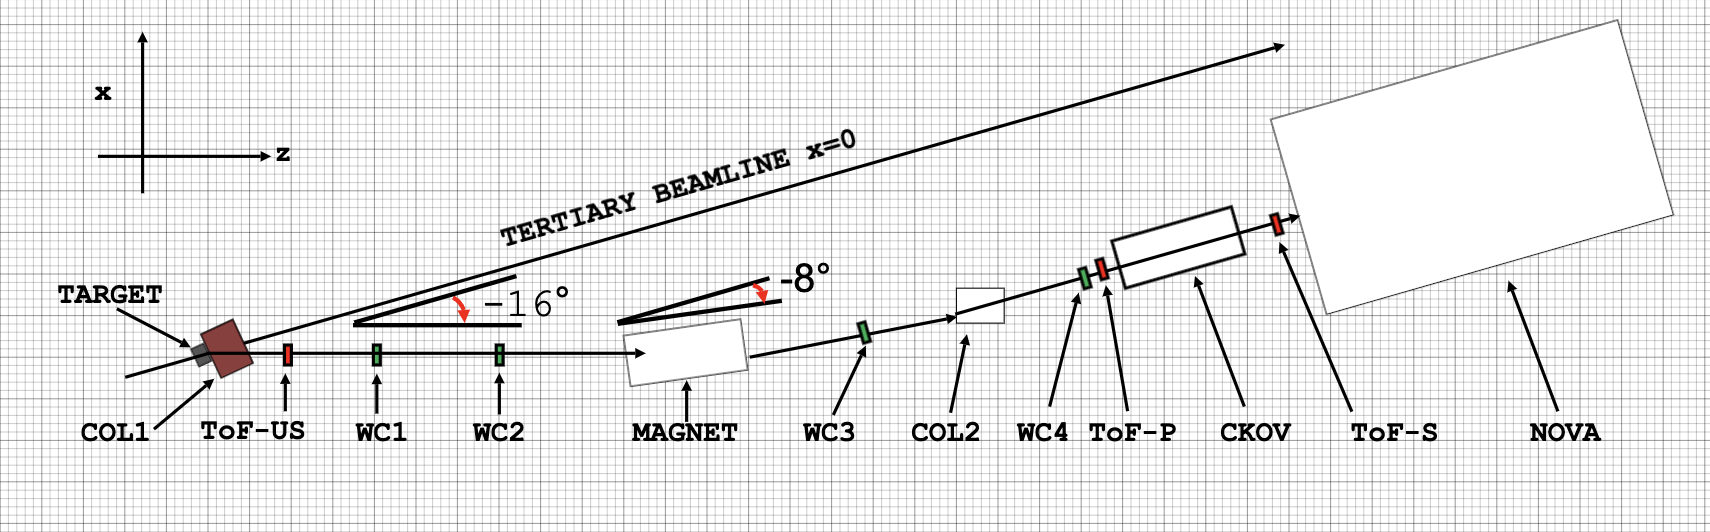
\includegraphics[scale=0.5]{overview.png}	 
   \caption[short]{A sketch of the beamline instrumentation as viewed from above.}
   \label{fig_overview}
  \end{figure}

\begin{figure}[h]	   
 \centering
        	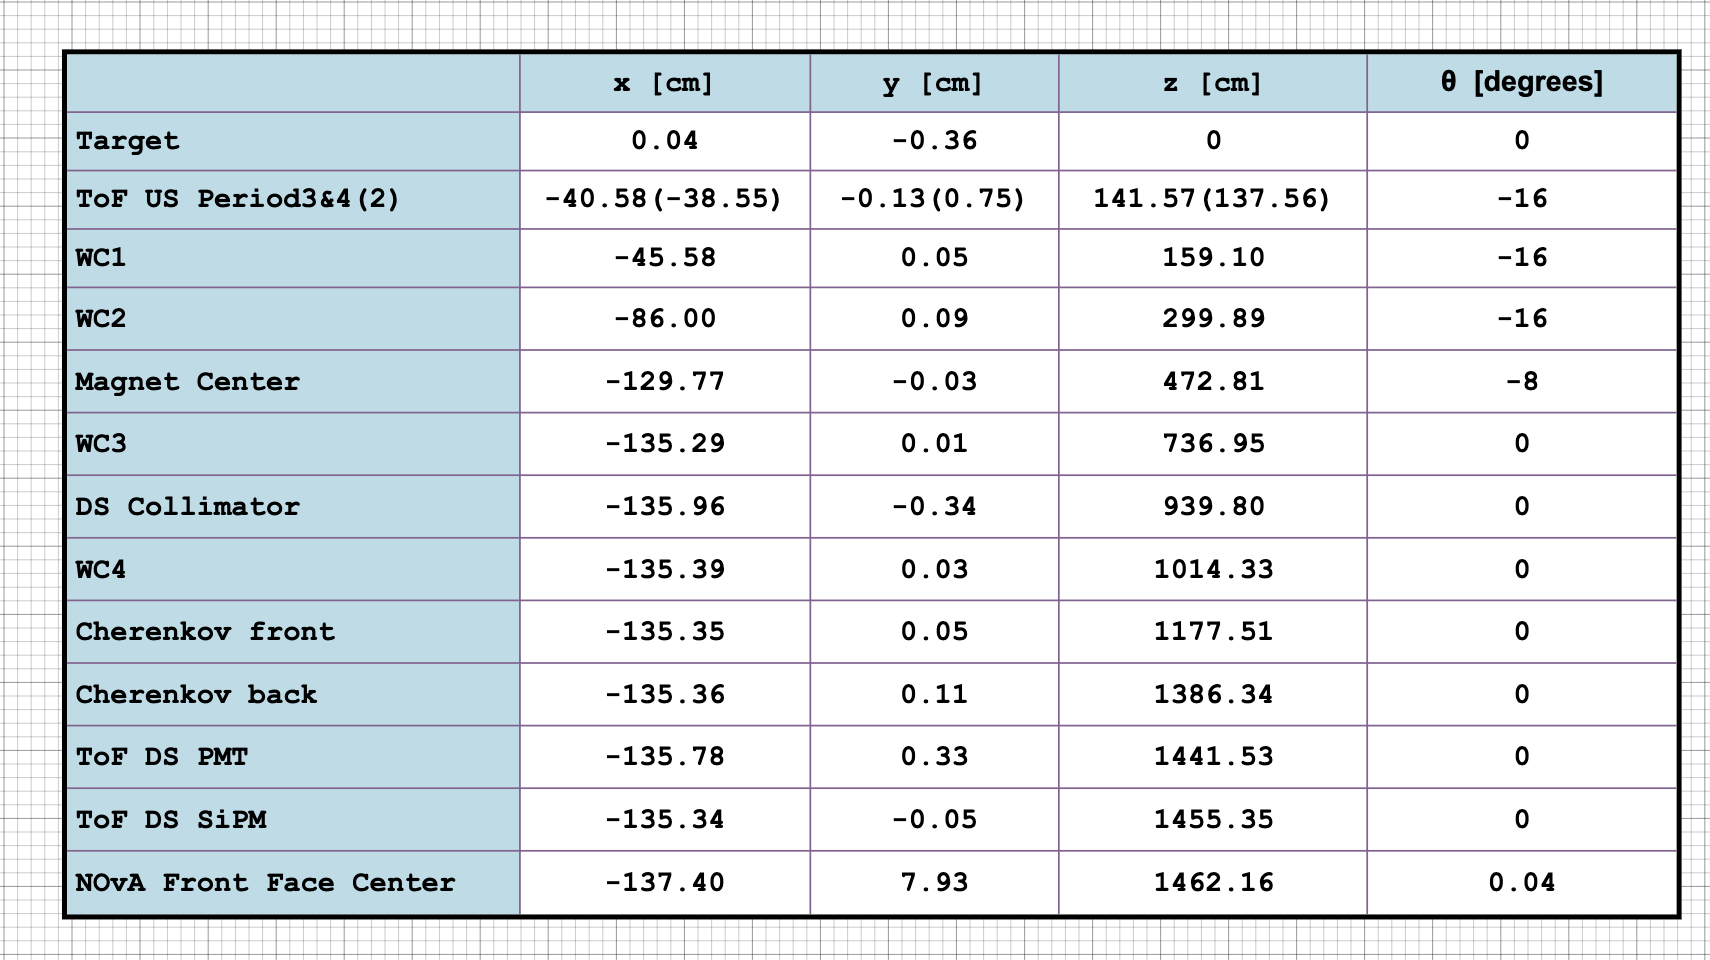
\includegraphics[scale=0.5]{coords.png}	 
   \caption[short]{Coordinates of some of the main components of the beamline instrumentation.}
   \label{fig_coords}
  \end{figure}
  
    \begin{figure}[h]	   
 \centering
        	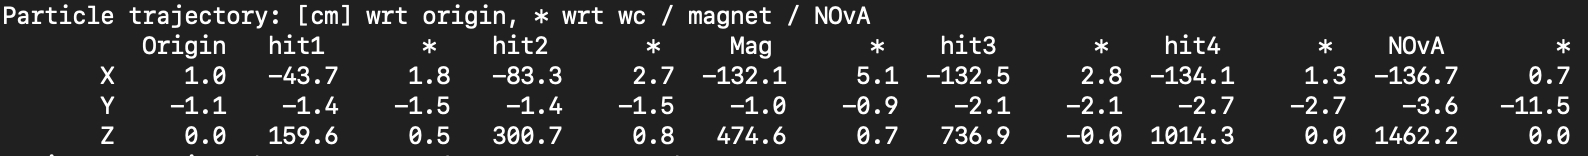
\includegraphics[scale=0.5]{example-traj.png}	 
   \caption[short]{An example trajectory of measurements along the beamline.}
   \label{fig_traj}
  \end{figure}
  
  
\subsection{The wirechamber coordinates}

Figure~\ref{fig_xyhits} show the hit positions in the four wirechambers. \textcolor{red}{The missing wires in WC1 increase over the periods of data taking, shown in Figure~\ref{fig_xyhitsperiod}}.

       \begin{figure}[h]	   
            \centering
   
            \begin{subfigure}[b]{0.23\textwidth}
            \centering
            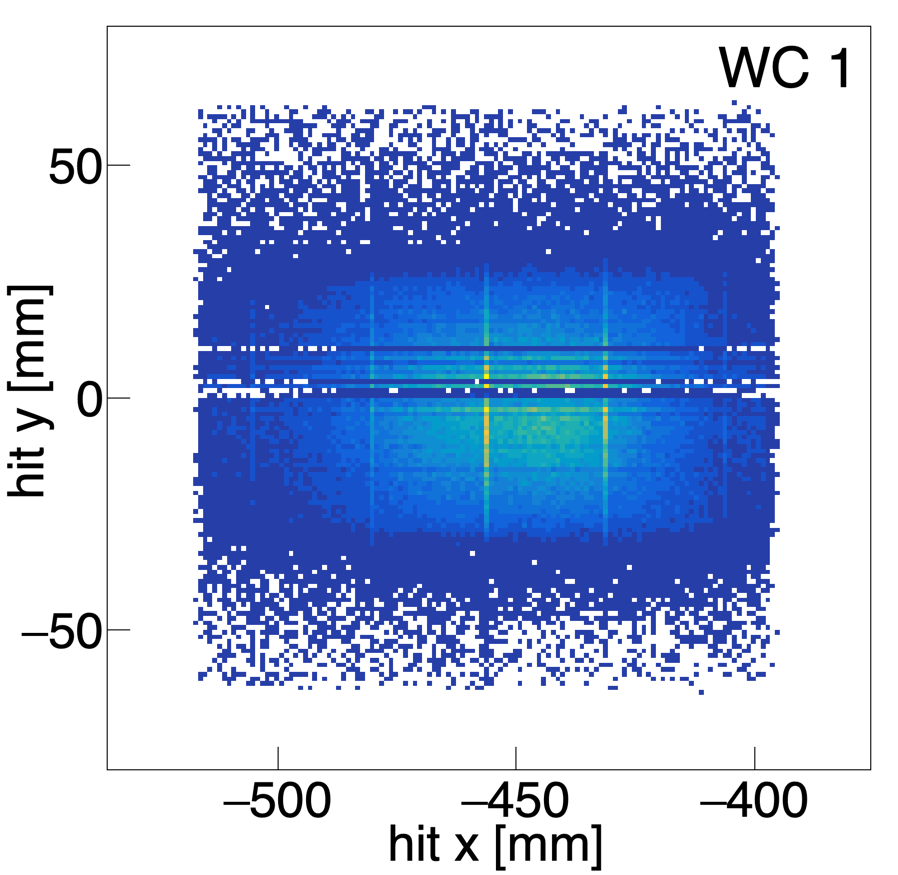
\includegraphics[width=\textwidth]{wcn_xy1_pol-1_period234.png}
            \caption{WC1}
            \label{fig_wc1}
            \end{subfigure}
            \hfill             
             \begin{subfigure}[b]{0.23\textwidth}
            \centering
            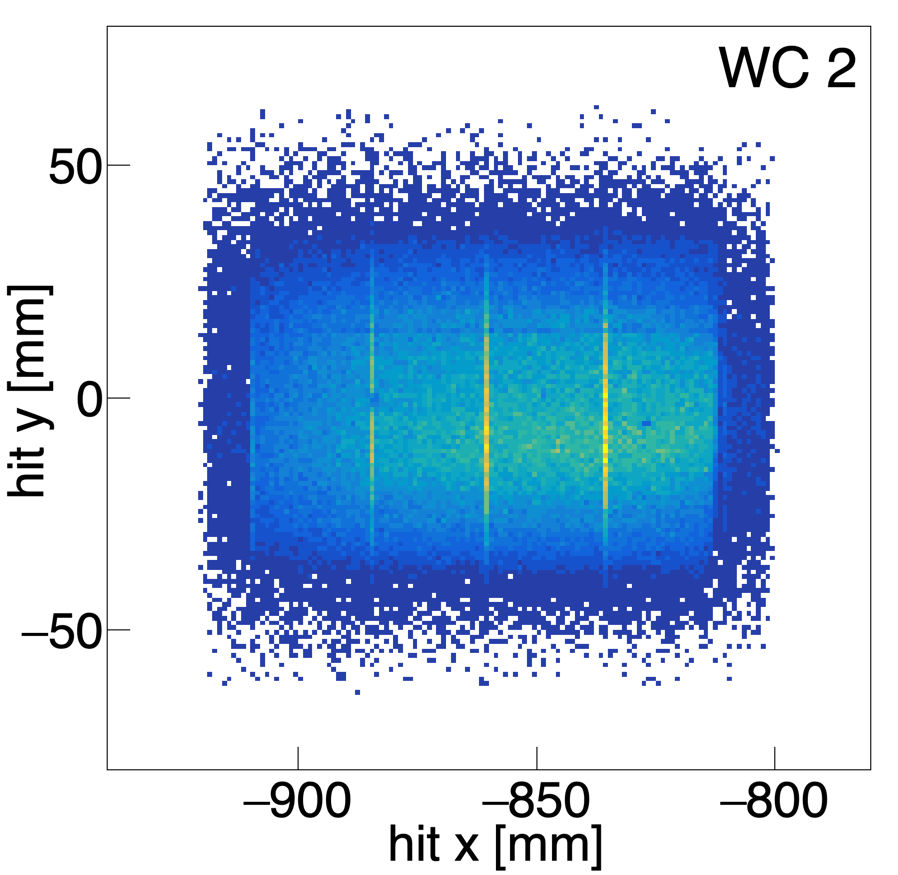
\includegraphics[width=\textwidth]{wcn_xy2_pol-1_period234.png}
            \caption{WC2}
            \label{fig_wc2}
            \end{subfigure}
            \hfill 
              \begin{subfigure}[b]{0.23\textwidth}
            \centering
            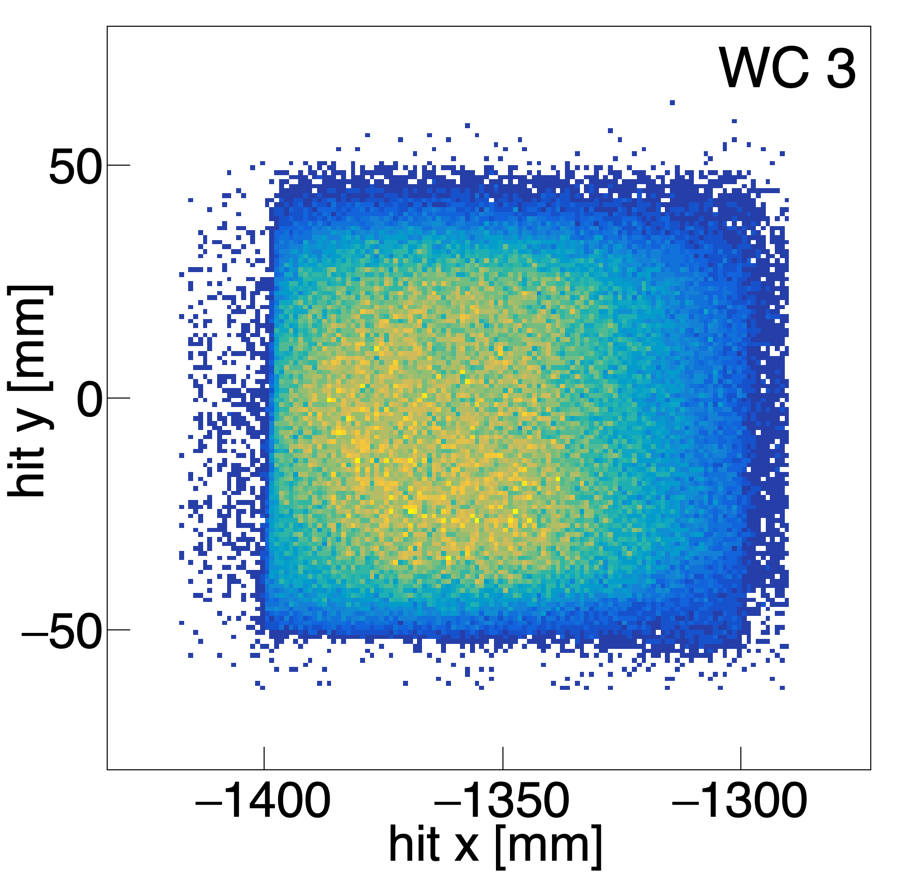
\includegraphics[width=\textwidth]{wcn_xy3_pol-1_period234.png}
            \caption{WC3}
            \label{fig_wc3}
            \end{subfigure}
            \hfill    
             \begin{subfigure}[b]{0.23\textwidth}
            \centering
            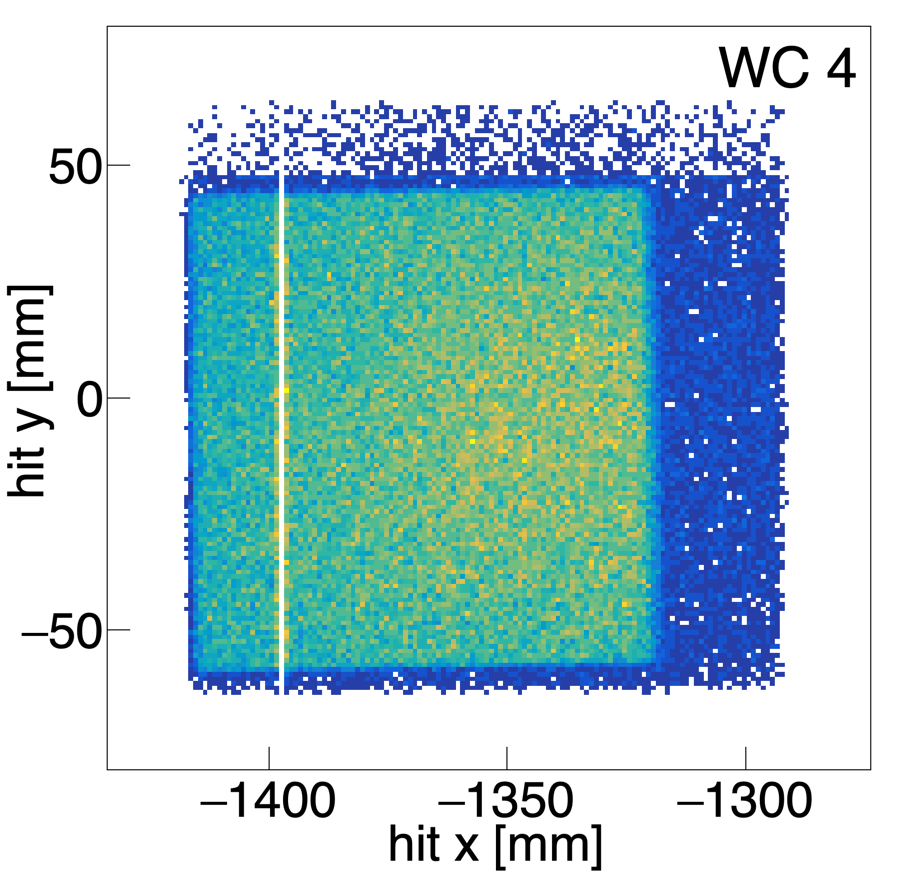
\includegraphics[width=\textwidth]{wcn_xy4_pol-1_period234.png}
            \caption{WC4}
            \label{fig_wc4}
            \end{subfigure}
            \hfill
   \caption[short]{The WCTrack best hit position in each of the four wire chambers, relative to the collimated tertiary beam. The best hit here means the hit that was attributed to the best track fit. Notice that wire chamber 1 has missing wires. All four hits must be present for these plots to be filled}
   \label{fig_xyhits}
  \end{figure}
  
  
         \begin{figure}[h]	   
            \centering
   	%miss 2
            \begin{subfigure}[b]{0.23\textwidth}
            \centering
            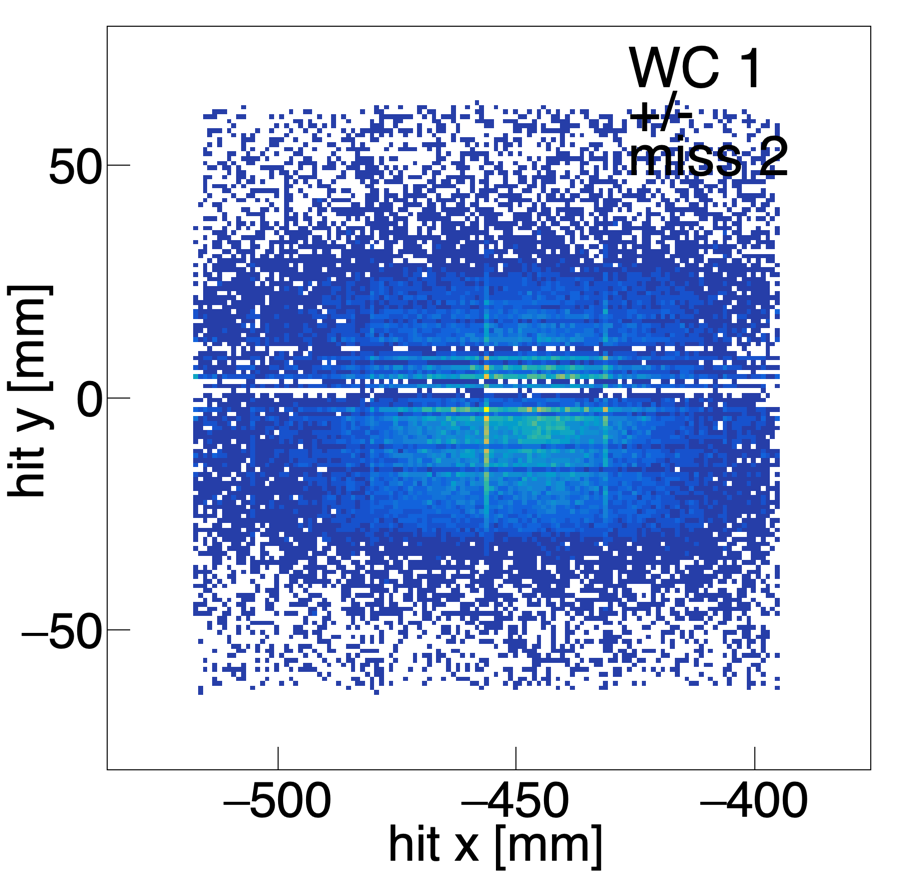
\includegraphics[width=\textwidth]{wcn_xy1_pol-1_period234_miss2.png}
            \caption{WC1, miss2}
            \label{fig_wc1}
            \end{subfigure}
            \hfill             
             \begin{subfigure}[b]{0.23\textwidth}
            \centering
            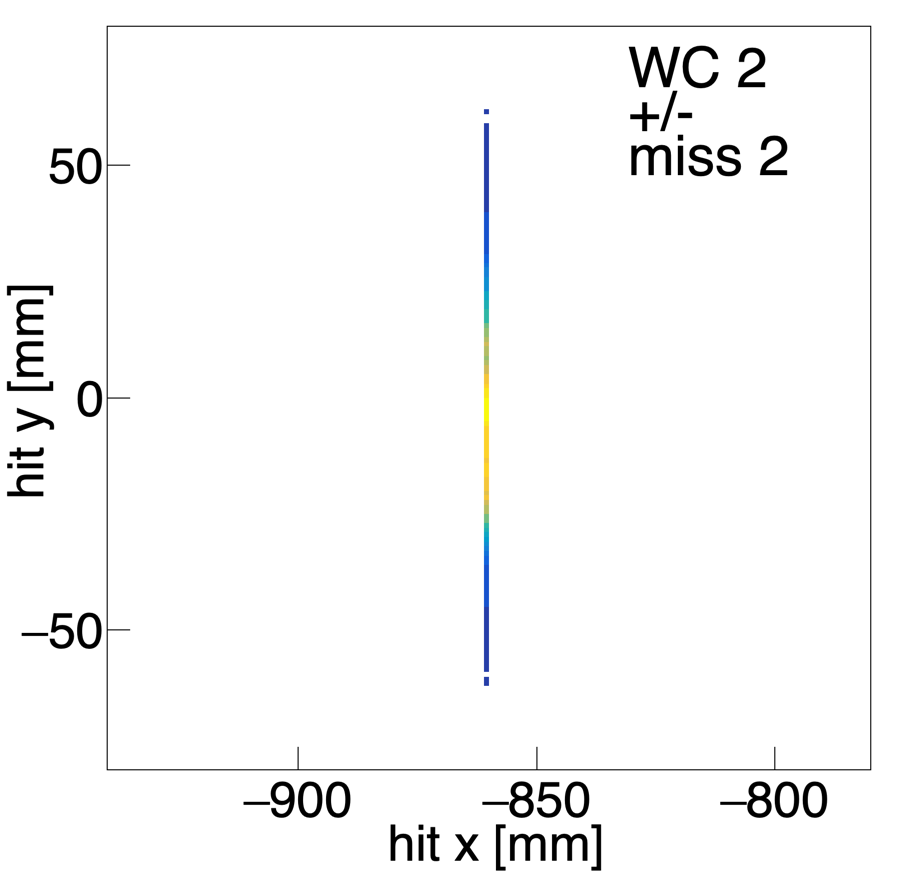
\includegraphics[width=\textwidth]{wcn_xy2_pol-1_period234_miss2.png}
            \caption{WC2, miss2}
            \label{fig_wc2}
            \end{subfigure}
            \hfill 
              \begin{subfigure}[b]{0.23\textwidth}
            \centering
            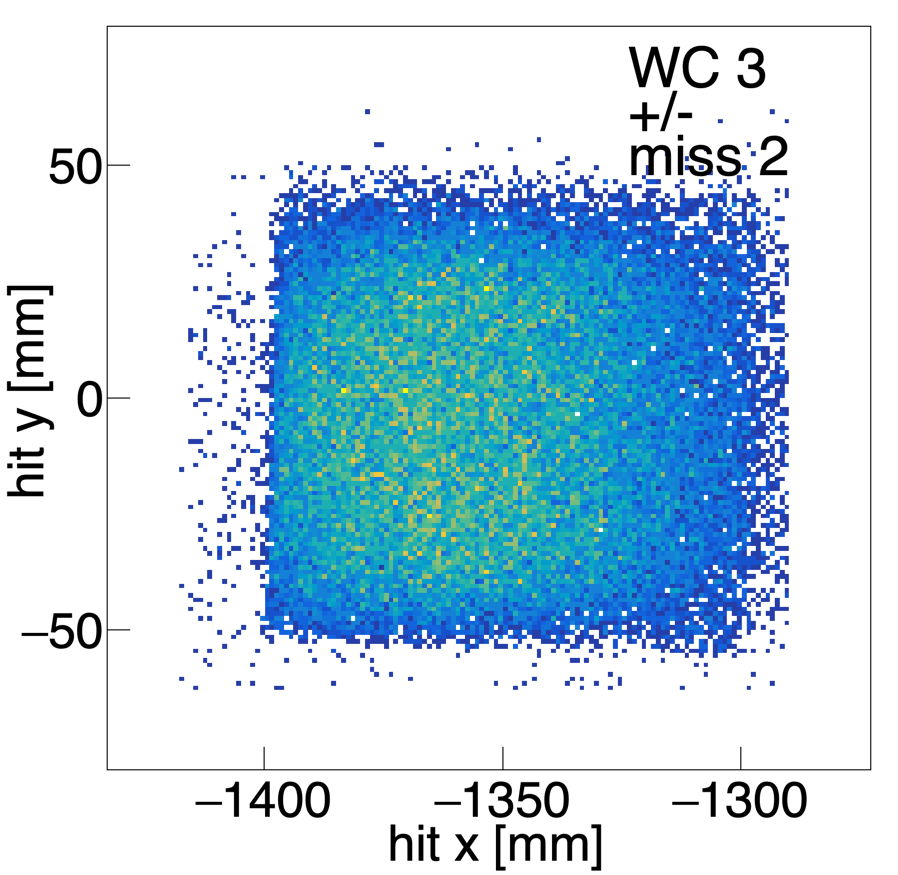
\includegraphics[width=\textwidth]{wcn_xy3_pol-1_period234_miss2.png}
            \caption{WC3, miss2}
            \label{fig_wc3}
            \end{subfigure}
            \hfill    
             \begin{subfigure}[b]{0.23\textwidth}
            \centering
            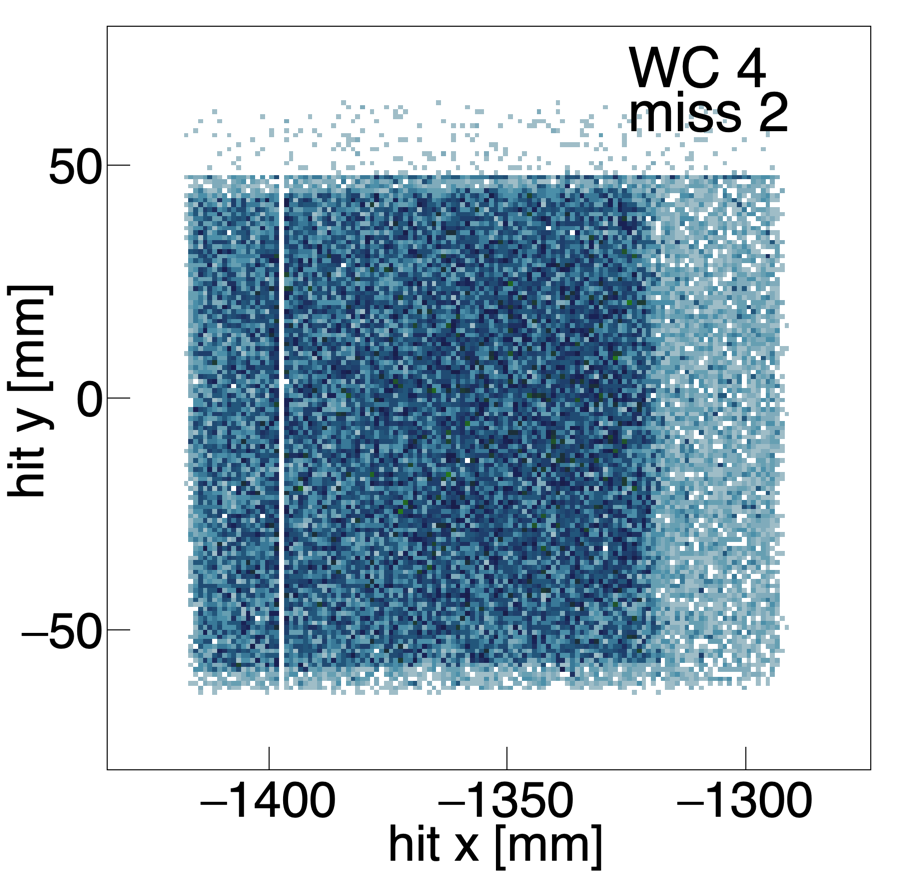
\includegraphics[width=\textwidth]{wcn_xy4_pol-1_period234_miss2.png}
            \caption{WC4, miss2}
            \label{fig_wc4}
            \end{subfigure}
            \hfill
            %miss3
                     \begin{subfigure}[b]{0.23\textwidth}
            \centering
            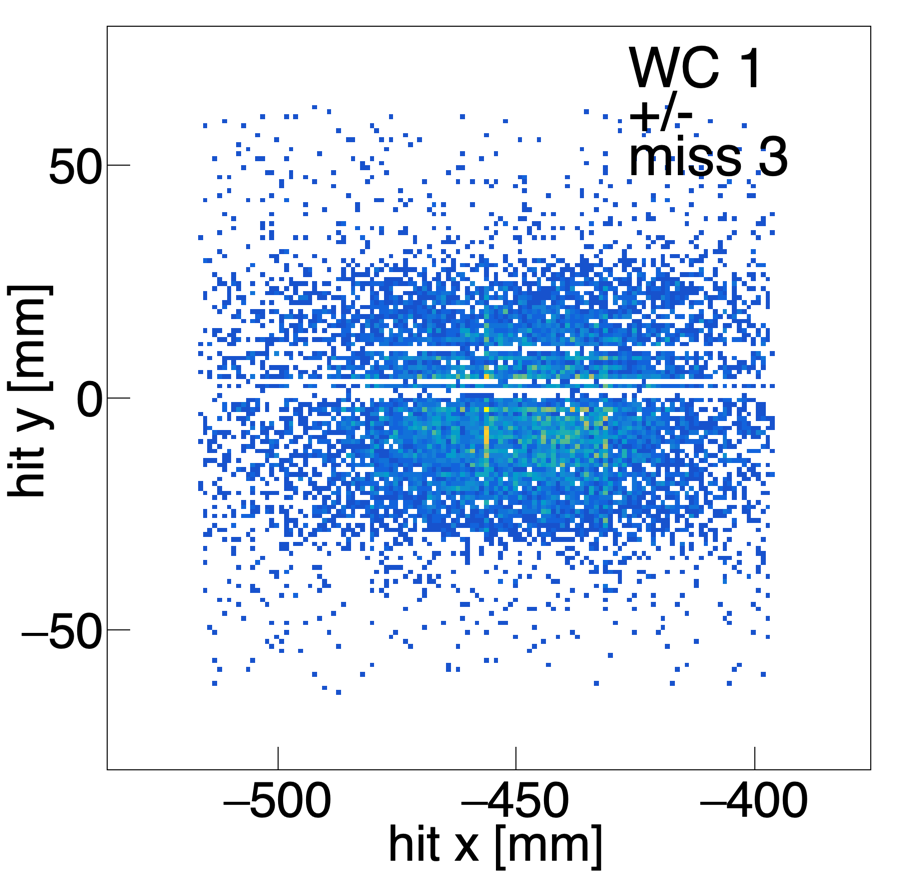
\includegraphics[width=\textwidth]{wcn_xy1_pol-1_period234_miss3.png}
            \caption{WC1, miss3}
            \label{fig_wc1}
            \end{subfigure}
            \hfill             
             \begin{subfigure}[b]{0.23\textwidth}
            \centering
            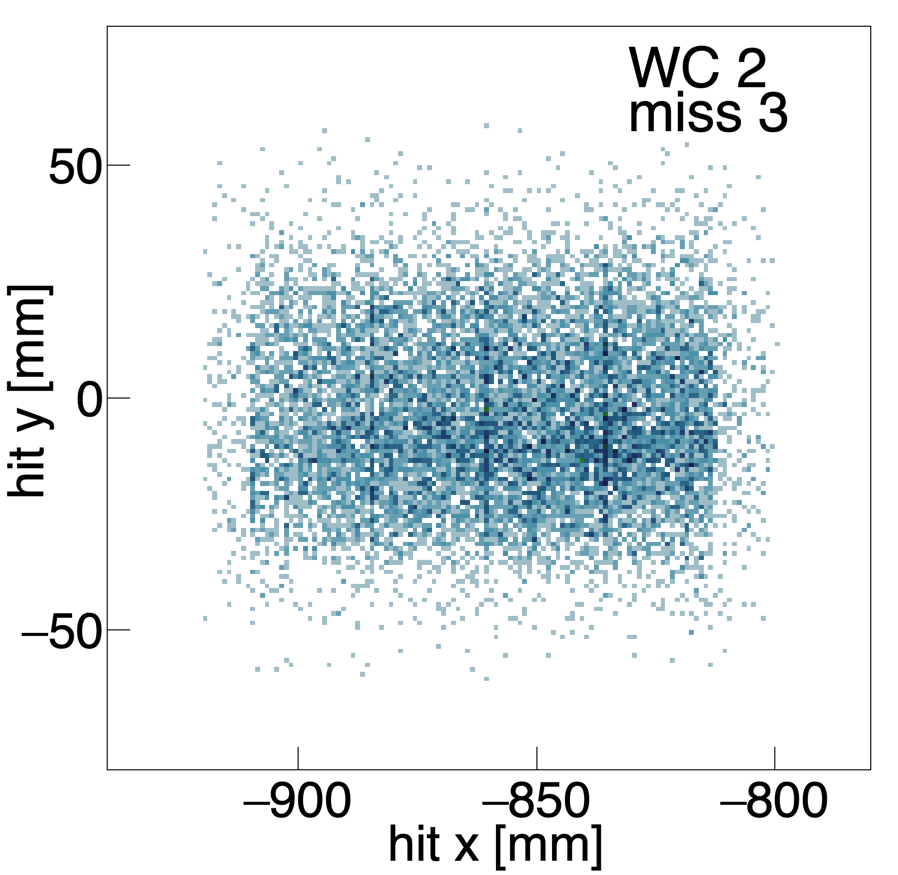
\includegraphics[width=\textwidth]{wcn_xy2_pol-1_period234_miss3.png}
            \caption{WC2, miss3}
            \label{fig_wc2}
            \end{subfigure}
            \hfill 
              \begin{subfigure}[b]{0.23\textwidth}
            \centering
            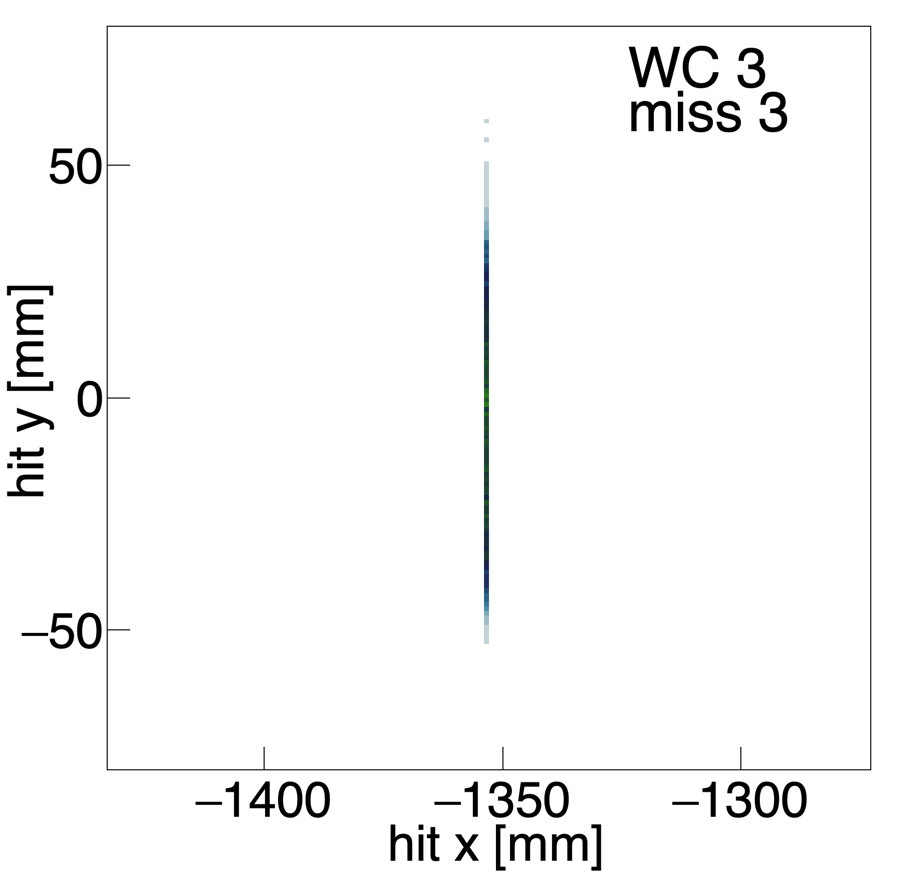
\includegraphics[width=\textwidth]{wcn_xy3_pol-1_period234_miss3.png}
            \caption{WC3, miss3}
            \label{fig_wc3}
            \end{subfigure}
            \hfill    
             \begin{subfigure}[b]{0.23\textwidth}
            \centering
            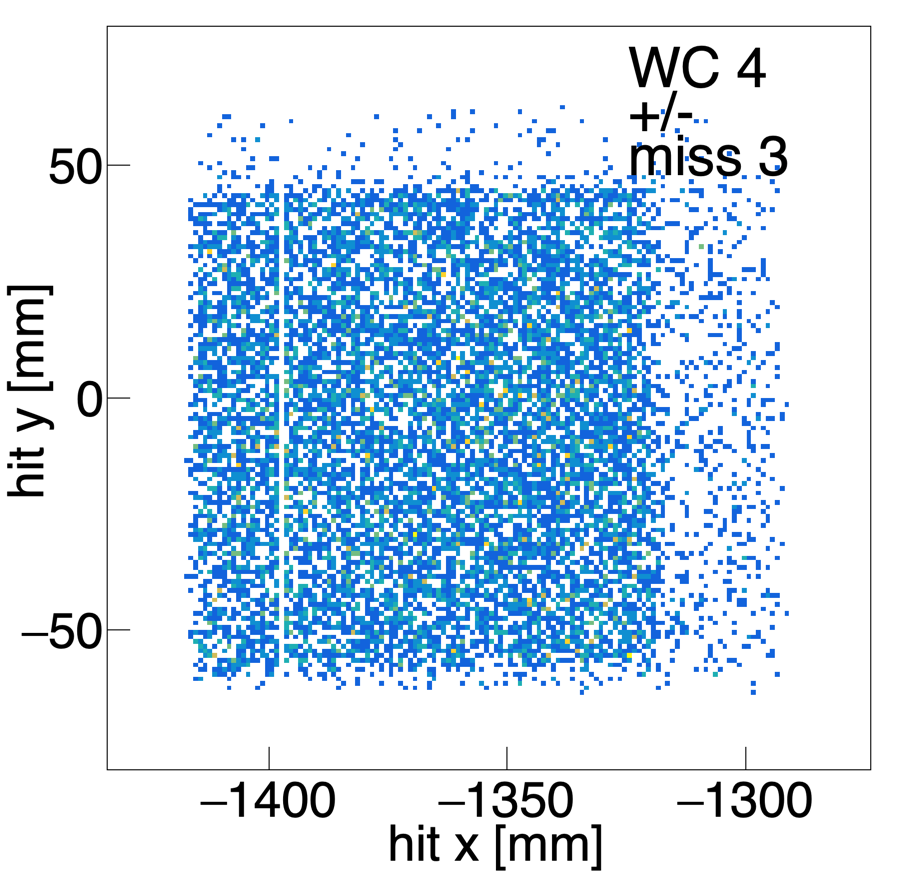
\includegraphics[width=\textwidth]{wcn_xy4_pol-1_period234_miss3.png}
            \caption{WC4, miss3}
            \label{fig_wc4}
            \end{subfigure}
            \hfill
            
             %miss3
                     \begin{subfigure}[b]{0.23\textwidth}
            \centering
            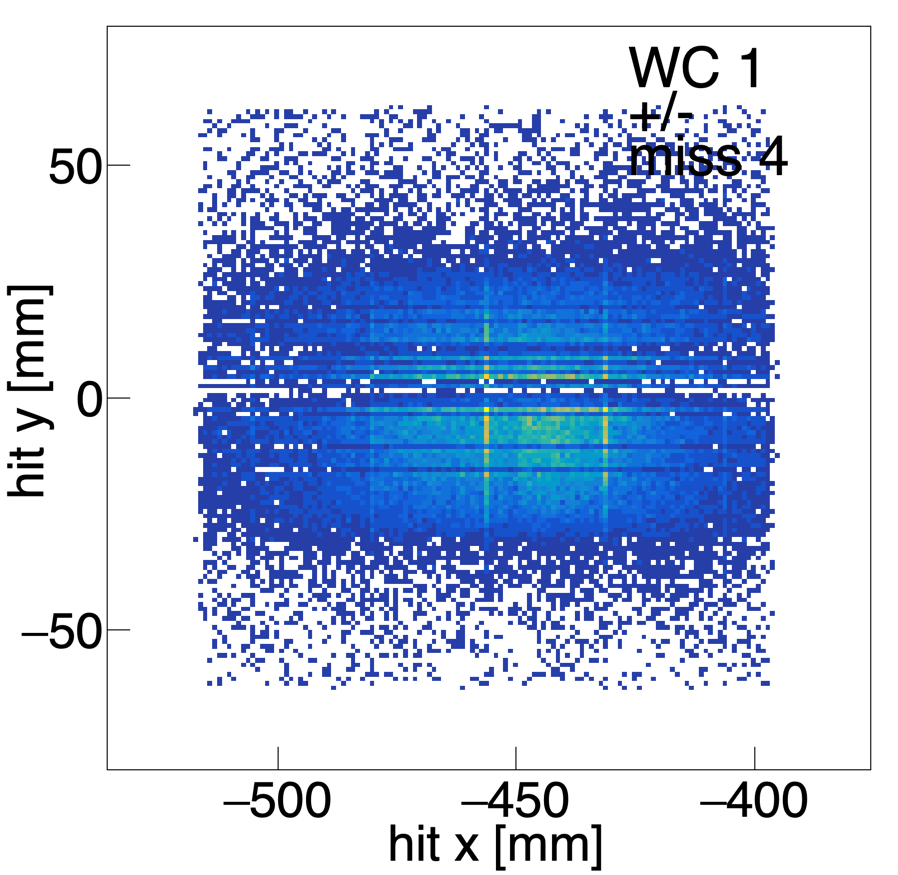
\includegraphics[width=\textwidth]{wcn_xy1_pol-1_period234_miss4.png}
            \caption{WC1, miss4}
            \label{fig_wc1}
            \end{subfigure}
            \hfill             
             \begin{subfigure}[b]{0.23\textwidth}
            \centering
            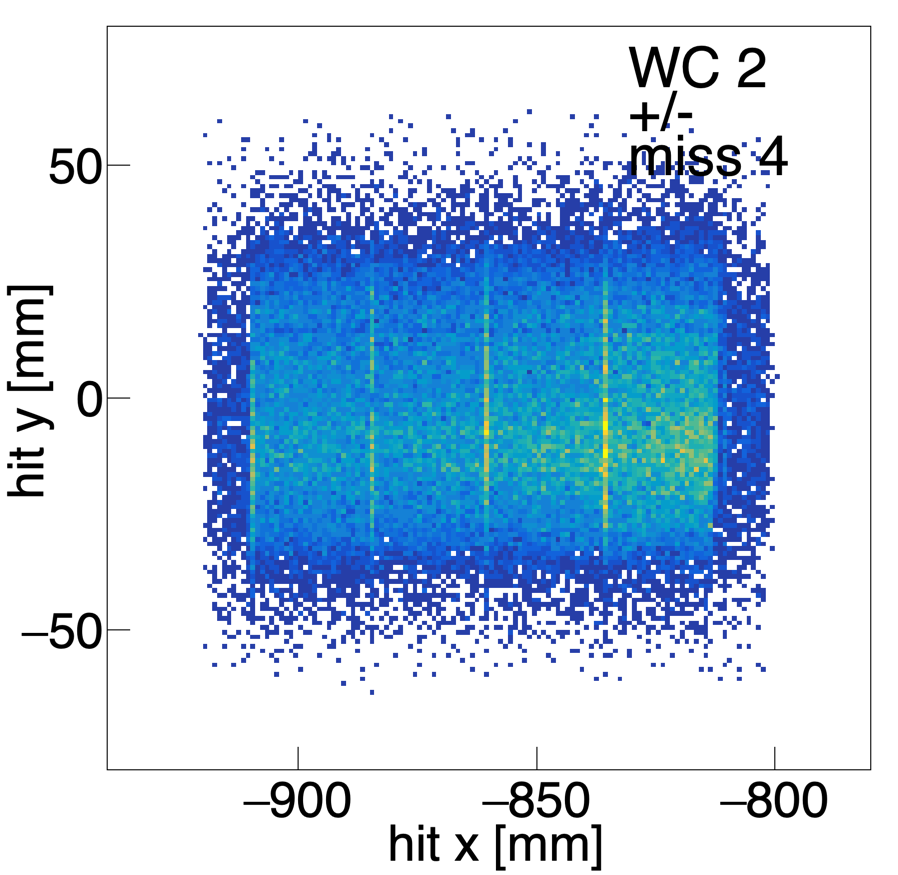
\includegraphics[width=\textwidth]{wcn_xy2_pol-1_period234_miss4.png}
            \caption{WC2, miss4}
            \label{fig_wc2}
            \end{subfigure}
            \hfill 
              \begin{subfigure}[b]{0.23\textwidth}
            \centering
            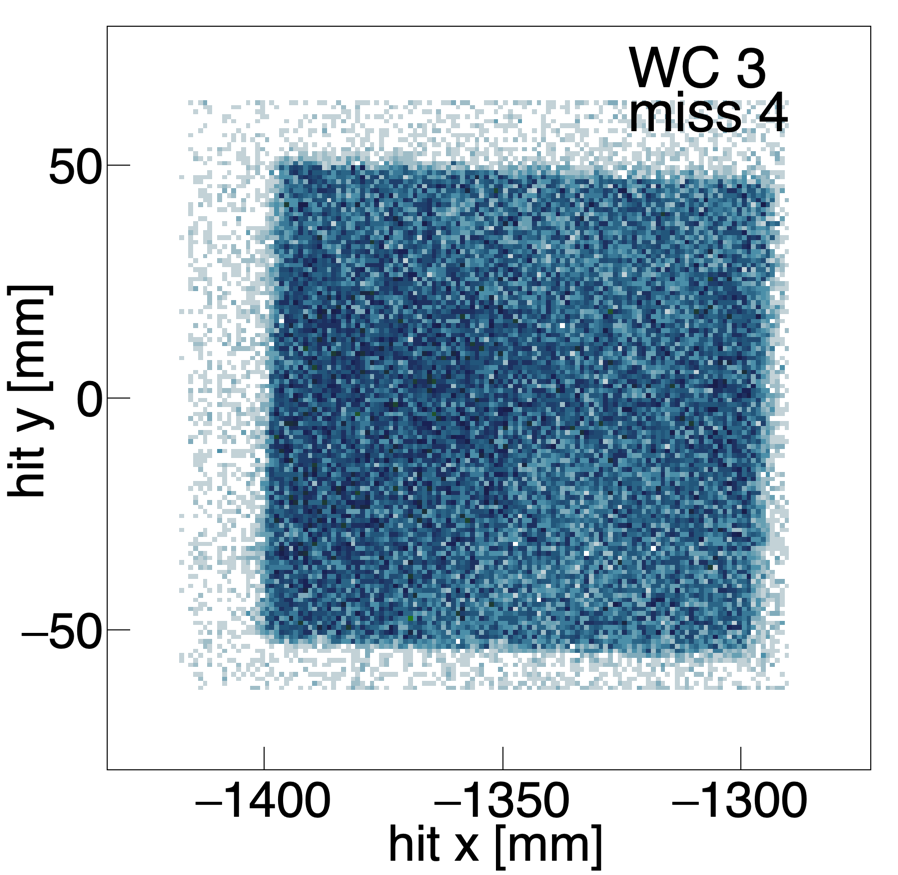
\includegraphics[width=\textwidth]{wcn_xy3_pol-1_period234_miss4.png}
            \caption{WC3, miss4}
            \label{fig_wc3}
            \end{subfigure}
            \hfill    
             \begin{subfigure}[b]{0.23\textwidth}
            \centering
            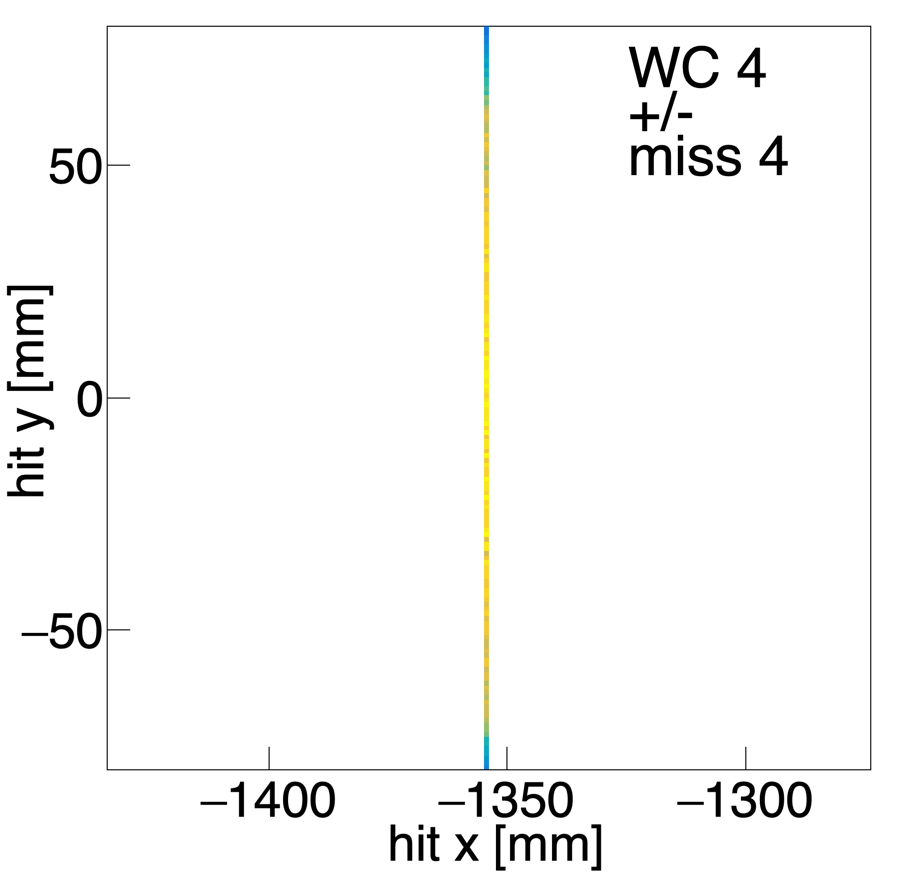
\includegraphics[width=\textwidth]{wcn_xy4_pol-1_period234_miss4.png}
            \caption{WC4, miss4}
            \label{fig_wc4}
            \end{subfigure}
            \hfill

   \caption[short]{The WCTrack best hit position in each of the four wire chambers, relative to the collimated tertiary beam. The best hit here means the hit that was attributed to the best track fit. Notice that wire chamber 1 has missing wires. Top row: tracks where the hit in wc2 is faked, middle row: hit 2 is faked, bottom row: hit 4 is faked.}
   \label{fig_xyhits}
  \end{figure}
  
  
  
  
  
         \begin{figure}[h]	   
            \centering
   
               \begin{subfigure}[b]{0.23\textwidth}
            \centering
            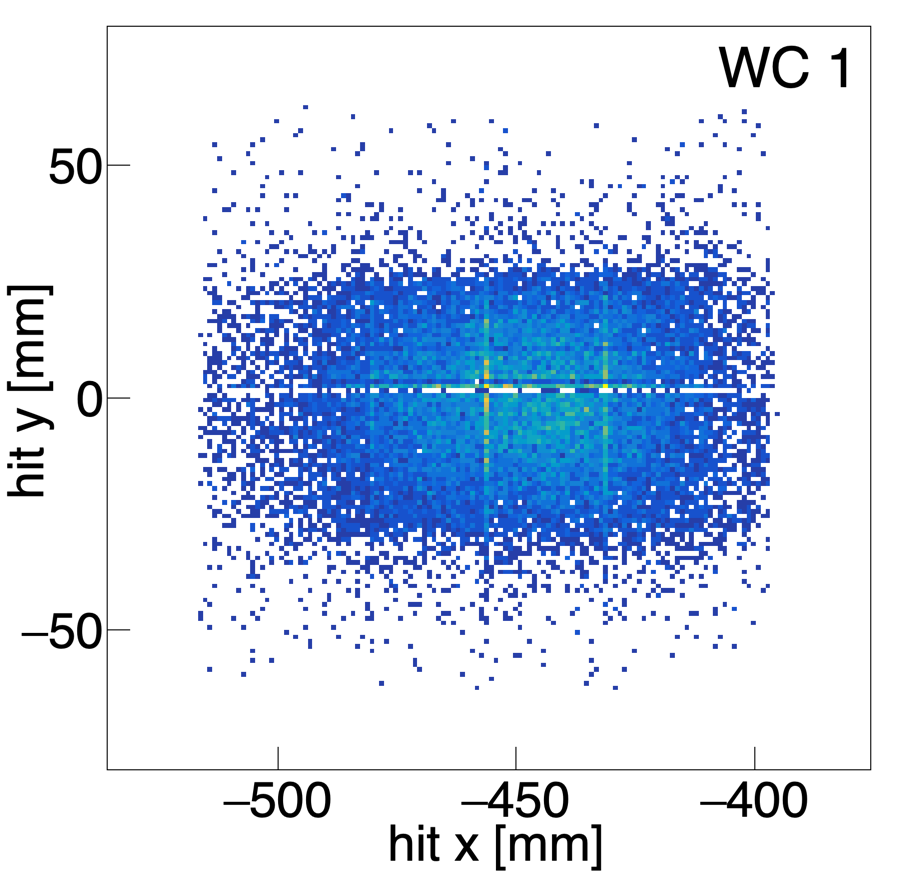
\includegraphics[width=\textwidth]{wcn_xy1_pol-1_period2.png}
            \caption{WC1, P2}
            \label{fig_wc1_p2}
            \end{subfigure}
            \hfill             
             \begin{subfigure}[b]{0.23\textwidth}
            \centering
            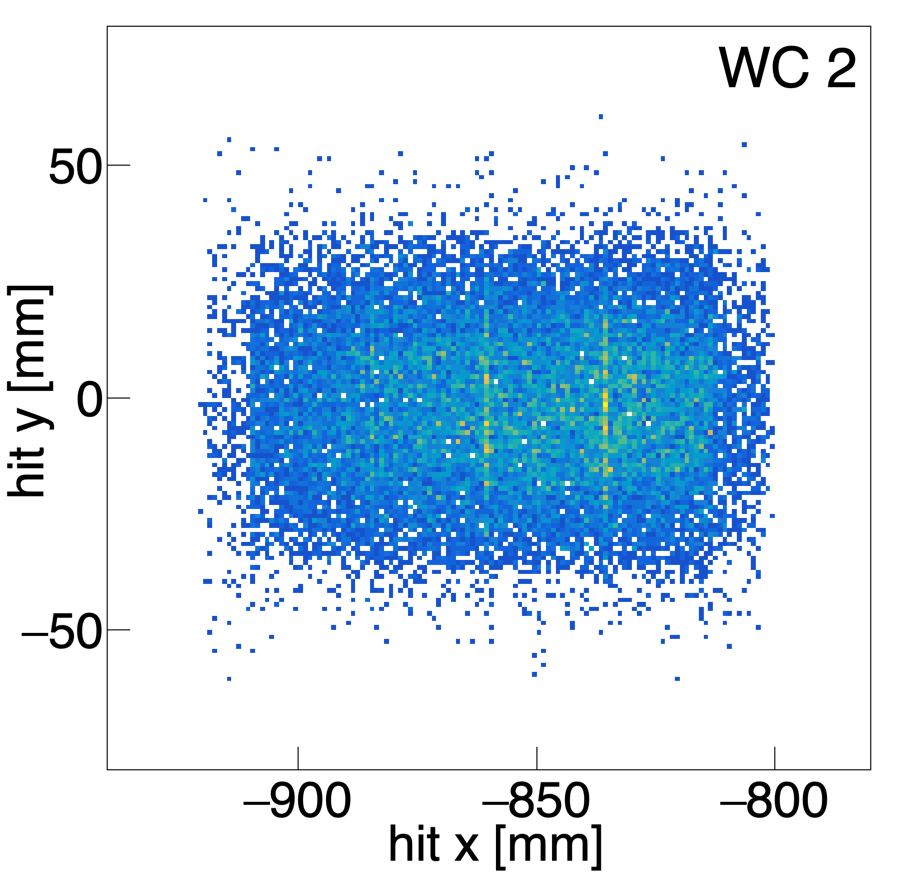
\includegraphics[width=\textwidth]{wcn_xy2_pol-1_period2.png}
            \caption{WC2, P2}
            \label{fig_wc2_p2}
            \end{subfigure}
            \hfill 
              \begin{subfigure}[b]{0.23\textwidth}
            \centering
            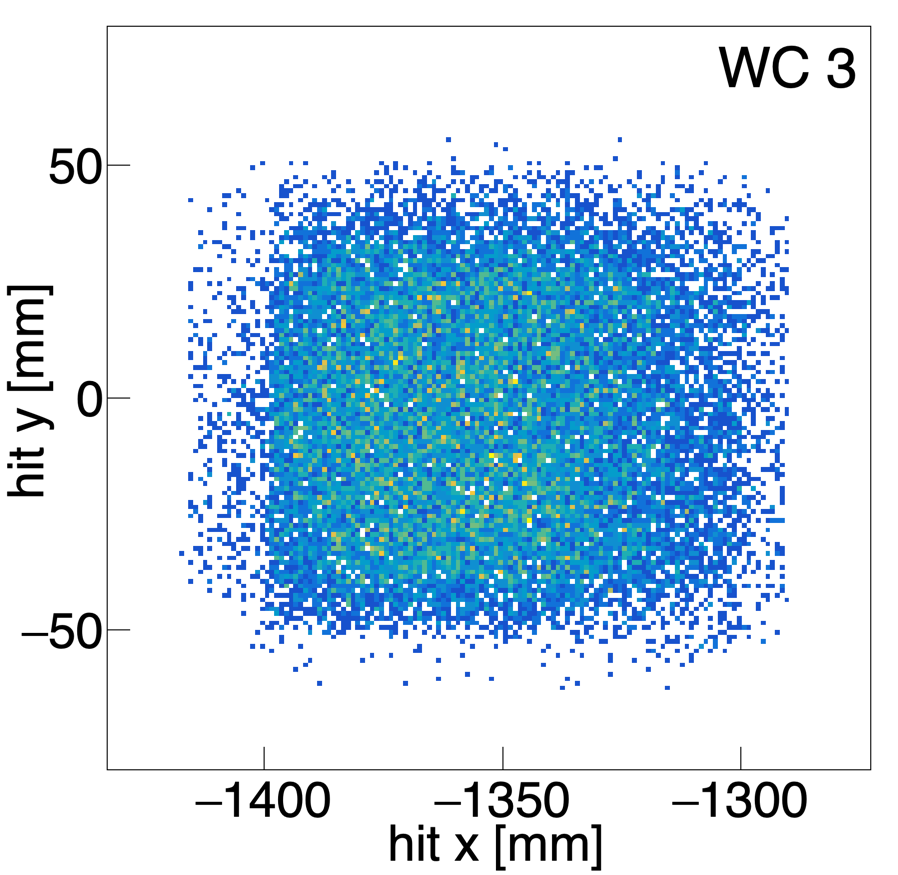
\includegraphics[width=\textwidth]{wcn_xy3_pol-1_period2.png}
            \caption{WC3, P2}
            \label{fig_wc3_p2}
            \end{subfigure}
            \hfill    
             \begin{subfigure}[b]{0.23\textwidth}
            \centering
            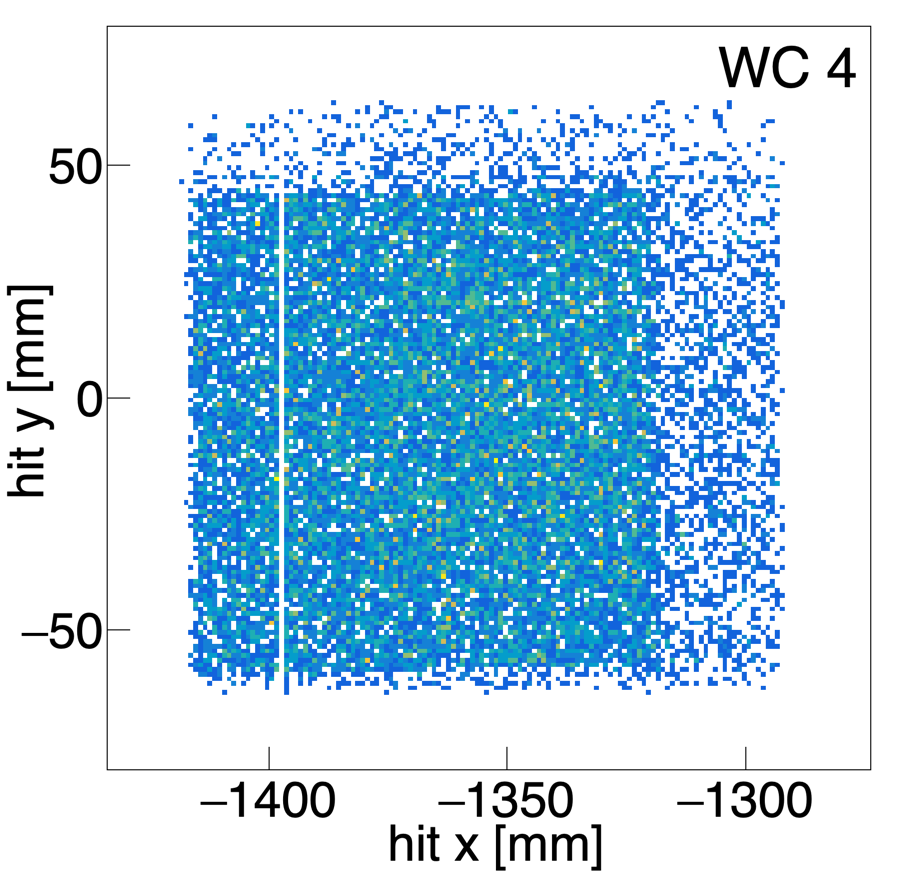
\includegraphics[width=\textwidth]{wcn_xy4_pol-1_period2.png}
            \caption{WC4, P2}
            \label{fig_wc4_p2}
            \end{subfigure}
            \hfill
   %p3
               \begin{subfigure}[b]{0.23\textwidth}
            \centering
            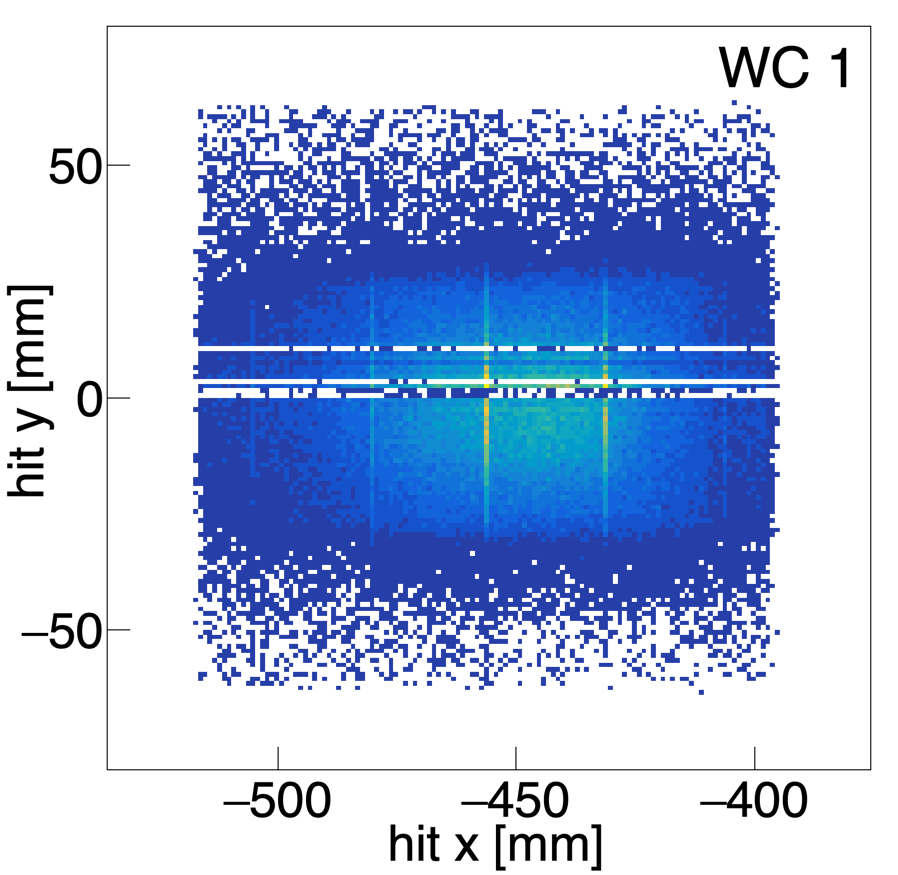
\includegraphics[width=\textwidth]{wcn_xy1_pol-1_period3.png}
            \caption{WC1, P3}
            \label{fig_wc1_p3}
            \end{subfigure}
            \hfill             
             \begin{subfigure}[b]{0.23\textwidth}
            \centering
            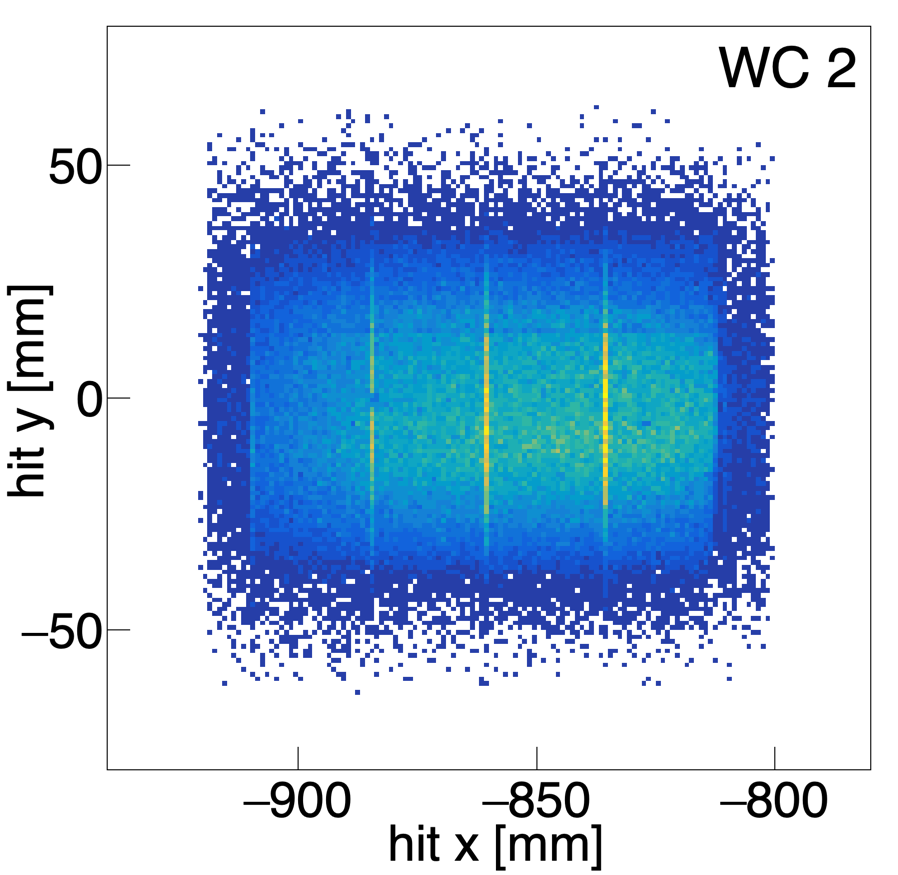
\includegraphics[width=\textwidth]{wcn_xy2_pol-1_period3.png}
            \caption{WC2, P3}
            \label{fig_wc2_p3}
            \end{subfigure}
            \hfill 
              \begin{subfigure}[b]{0.23\textwidth}
            \centering
            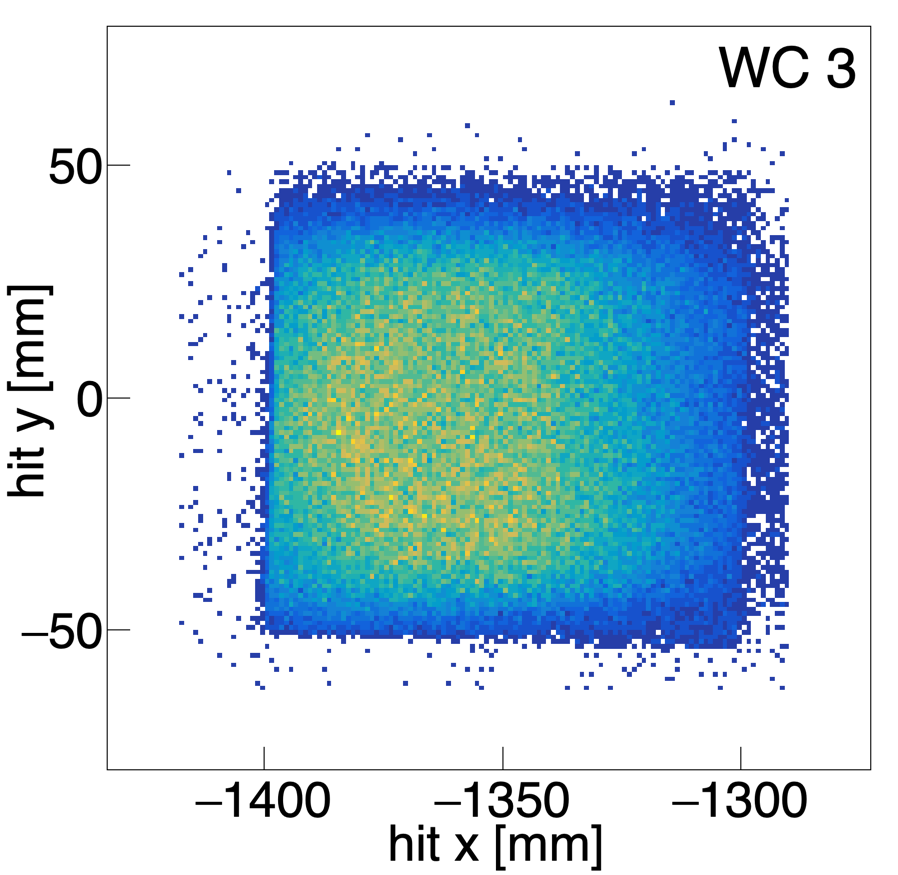
\includegraphics[width=\textwidth]{wcn_xy3_pol-1_period3.png}
            \caption{WC3, P3}
            \label{fig_wc3_p3}
            \end{subfigure}
            \hfill    
             \begin{subfigure}[b]{0.23\textwidth}
            \centering
            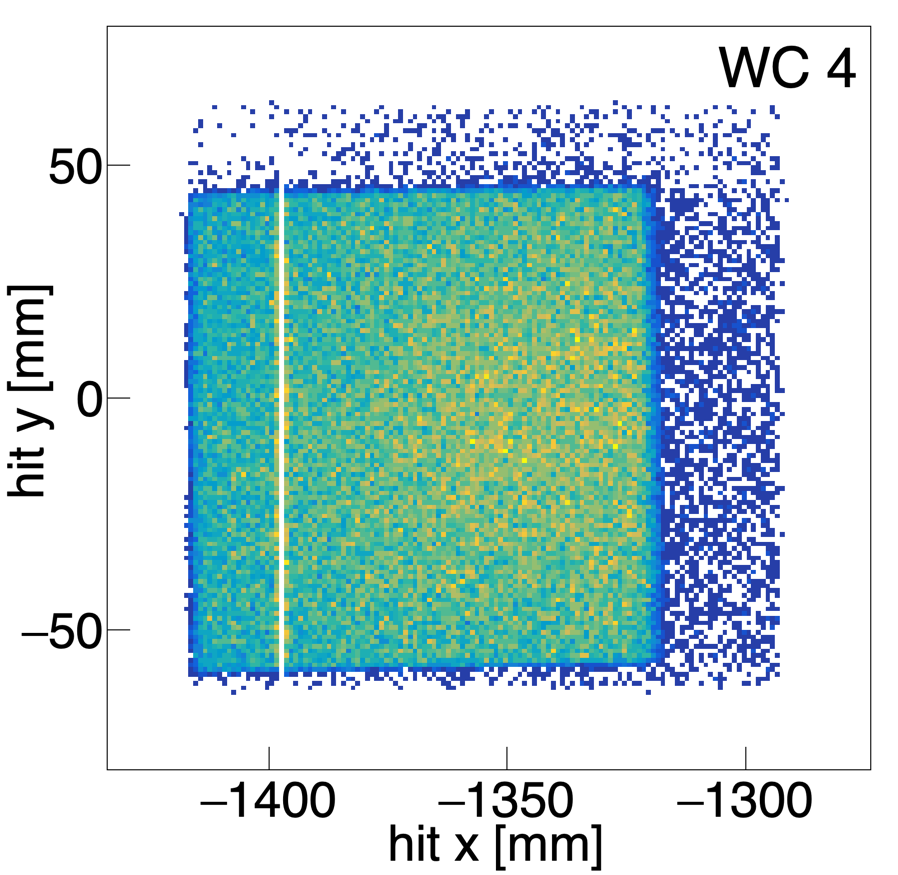
\includegraphics[width=\textwidth]{wcn_xy4_pol-1_period3.png}
            \caption{WC4, P3}
            \label{fig_wc4_p3}
            \end{subfigure}
            \hfill
   %p4
            \begin{subfigure}[b]{0.23\textwidth}
            \centering
            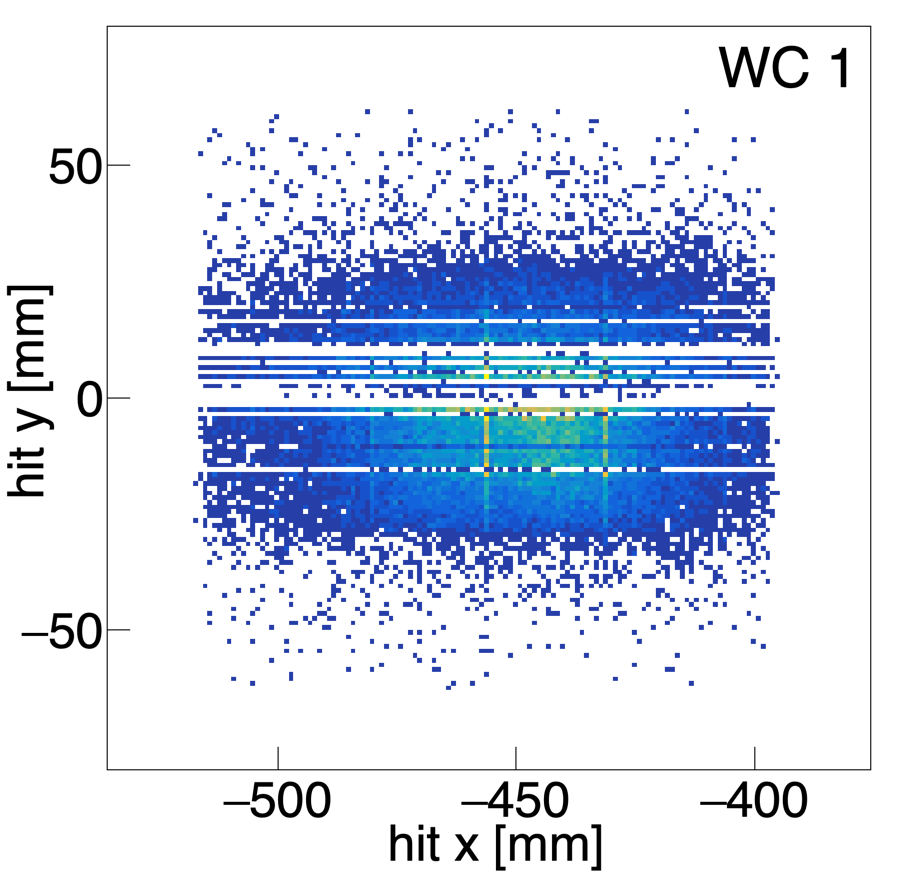
\includegraphics[width=\textwidth]{wcn_xy1_pol-1_period4.png}
            \caption{WC1, P4}
            \label{fig_wc1_p4}
            \end{subfigure}
            \hfill             
             \begin{subfigure}[b]{0.23\textwidth}
            \centering
            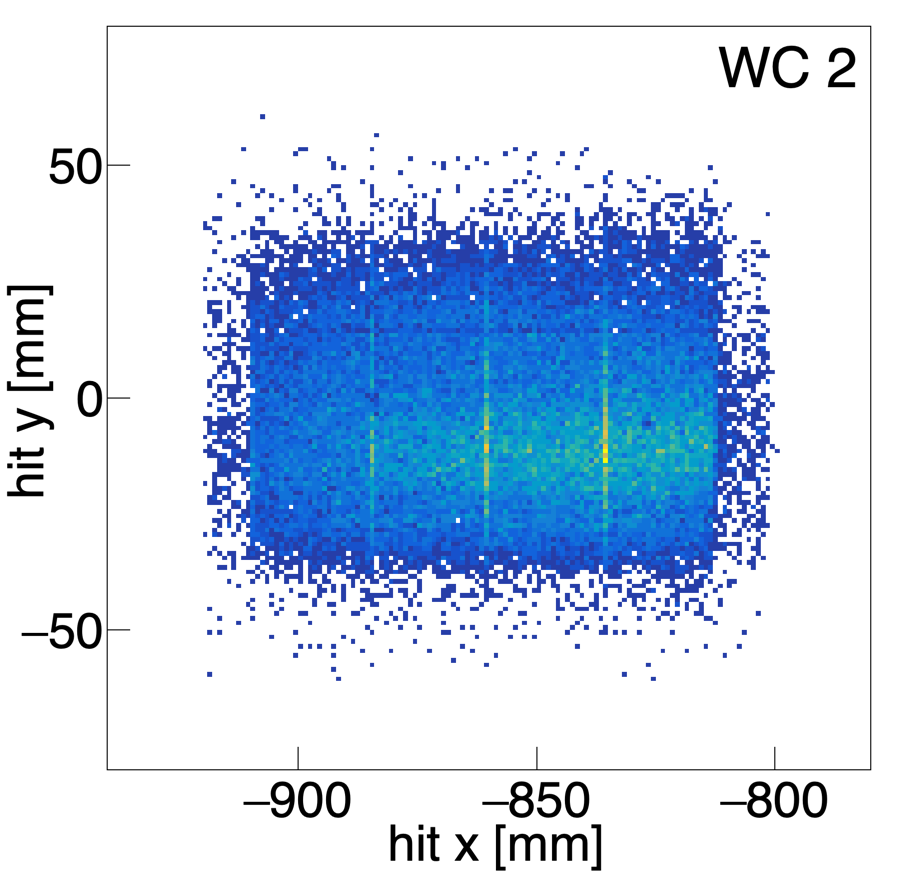
\includegraphics[width=\textwidth]{wcn_xy2_pol-1_period4.png}
            \caption{WC2, P4}
            \label{fig_wc2_p4}
            \end{subfigure}
            \hfill 
              \begin{subfigure}[b]{0.23\textwidth}
            \centering
            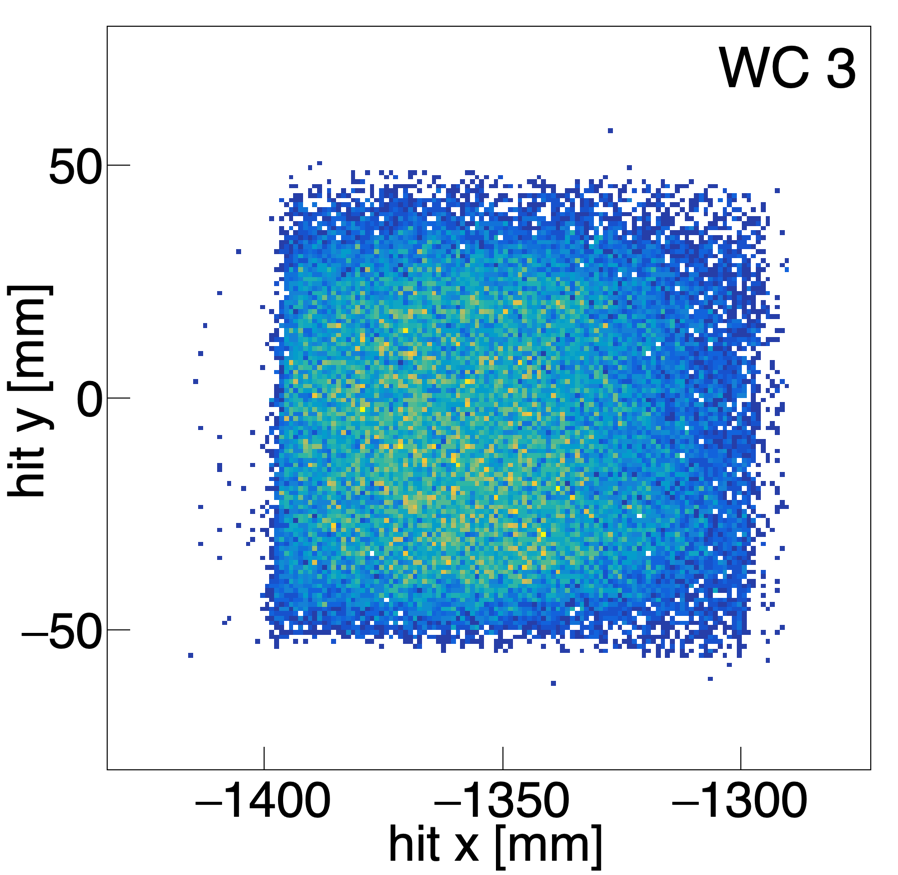
\includegraphics[width=\textwidth]{wcn_xy3_pol-1_period4.png}
            \caption{WC3, P4}
            \label{fig_wc3_p4}
            \end{subfigure}
            \hfill    
             \begin{subfigure}[b]{0.23\textwidth}
            \centering
            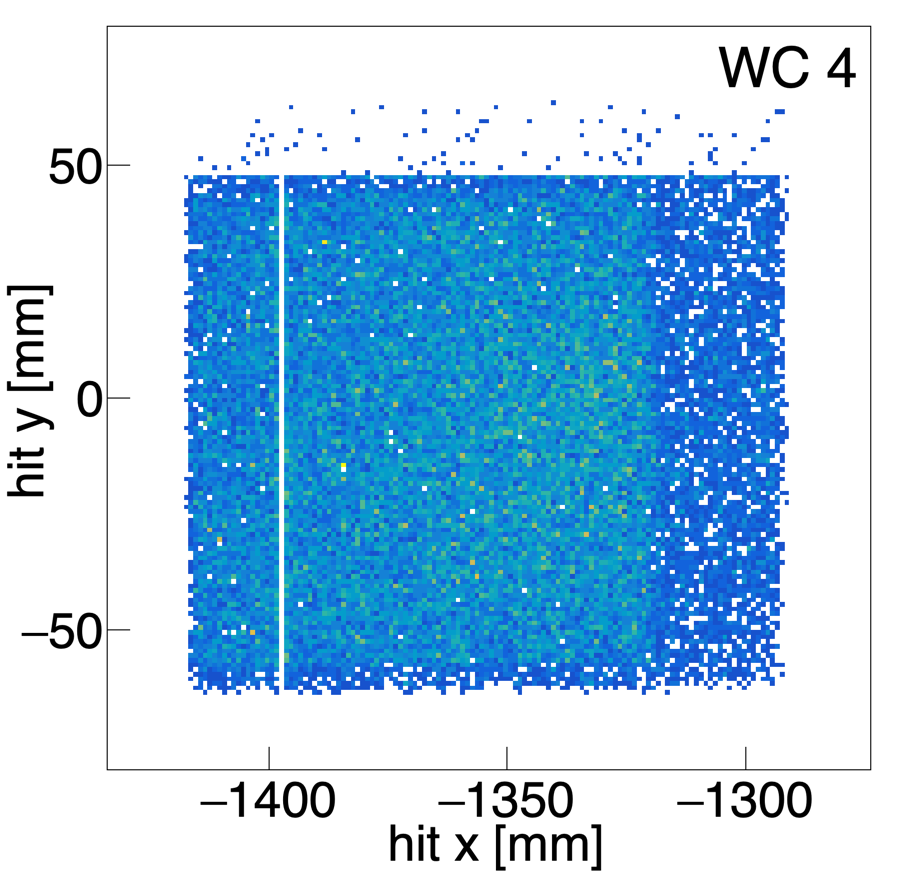
\includegraphics[width=\textwidth]{wcn_xy4_pol-1_period4.png}
            \caption{WC4, P4}
            \label{fig_wc4_p4}
            \end{subfigure}
            \hfill
   \caption[short]{The WCTrack best hit position in each of the four wire chambers, divided by period.}
   \label{fig_xyhitsperiod}
  \end{figure}
  
  
  
           \begin{figure}[h]	   
            \centering
   
               \begin{subfigure}[b]{0.23\textwidth}
            \centering
            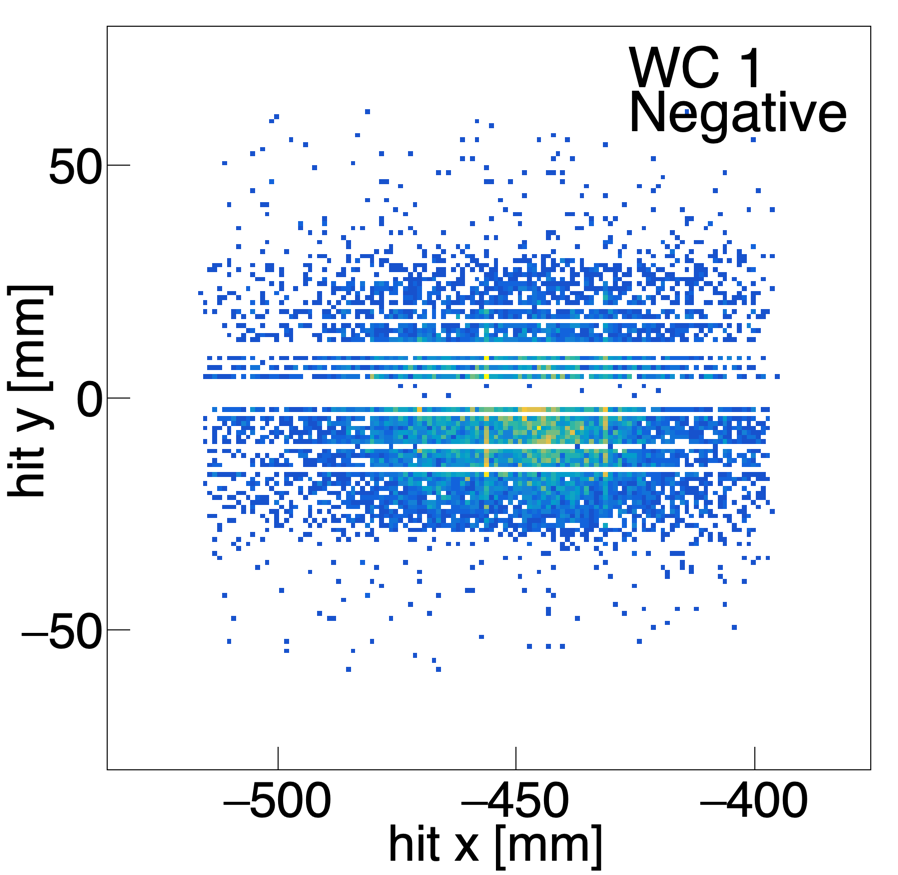
\includegraphics[width=\textwidth]{wcn_xy1_pol0_period4.png}
            \caption{WC1, P3}
            \label{fig_wc1_p3}
            \end{subfigure}
            \hfill             
             \begin{subfigure}[b]{0.23\textwidth}
            \centering
            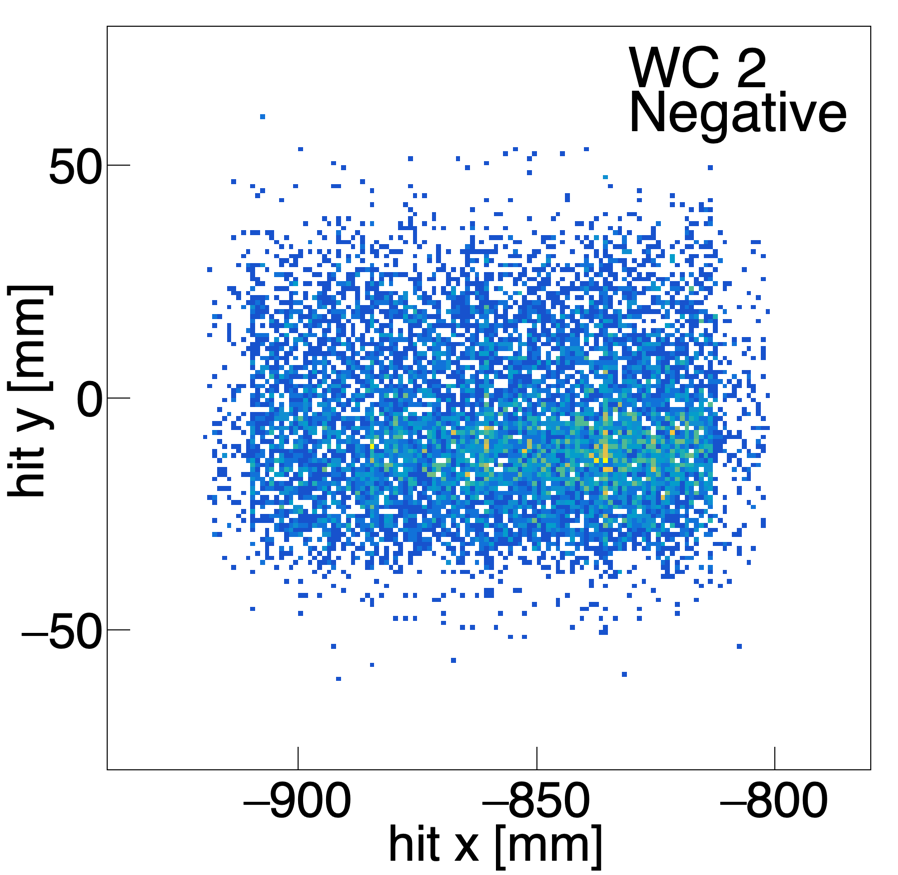
\includegraphics[width=\textwidth]{wcn_xy2_pol0_period4.png}
            \caption{WC2, P3}
            \label{fig_wc2_p3}
            \end{subfigure}
            \hfill 
              \begin{subfigure}[b]{0.23\textwidth}
            \centering
            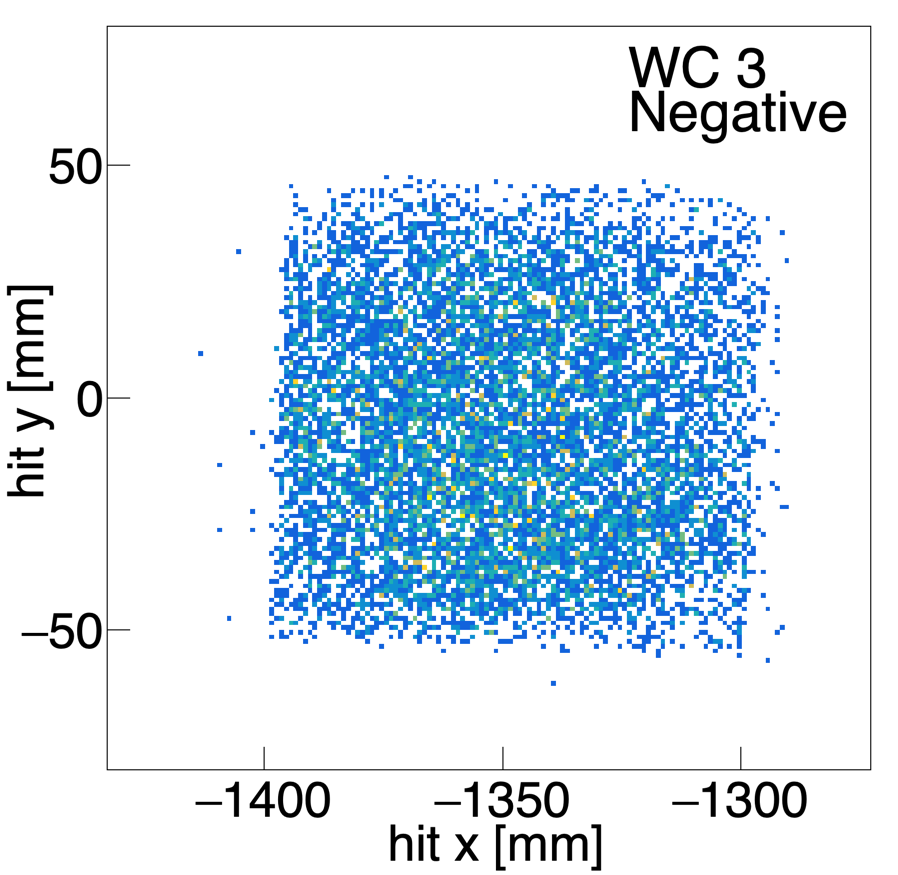
\includegraphics[width=\textwidth]{wcn_xy3_pol0_period4.png}
            \caption{WC3, P3}
            \label{fig_wc3_p3}
            \end{subfigure}
            \hfill    
             \begin{subfigure}[b]{0.23\textwidth}
            \centering
            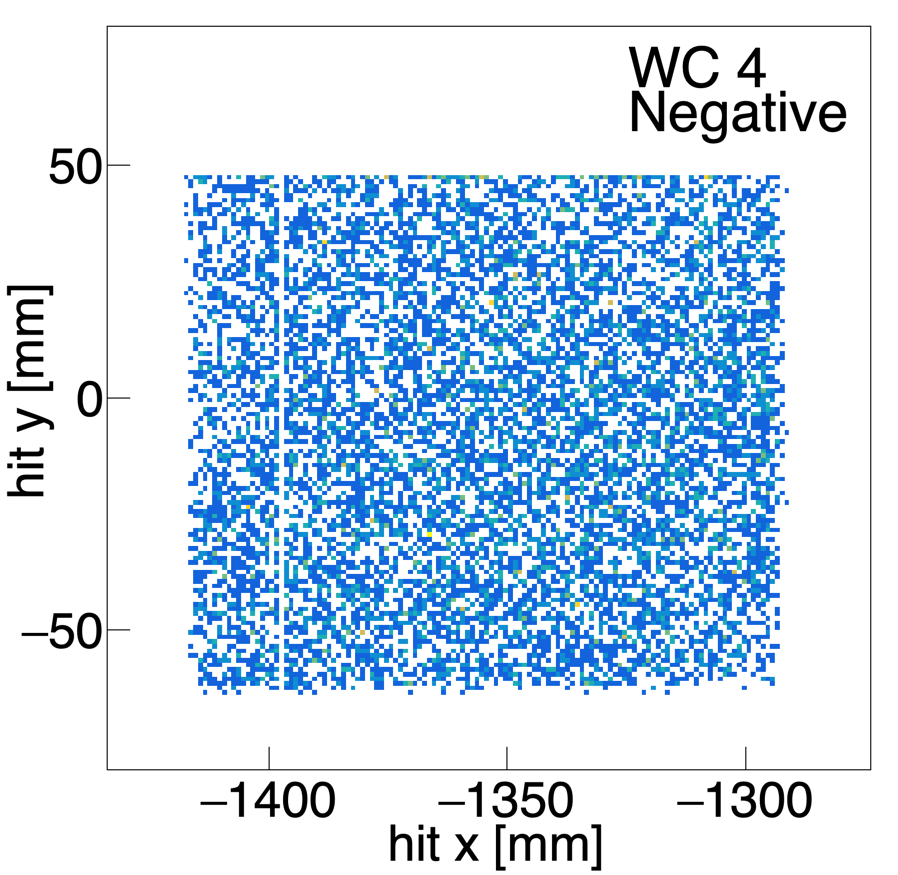
\includegraphics[width=\textwidth]{wcn_xy4_pol0_period4.png}
            \caption{WC4, P4, Negative}
            \label{fig_wc4_p3}
            \end{subfigure}
            \hfill
   %p4 positive
            \begin{subfigure}[b]{0.23\textwidth}
            \centering
            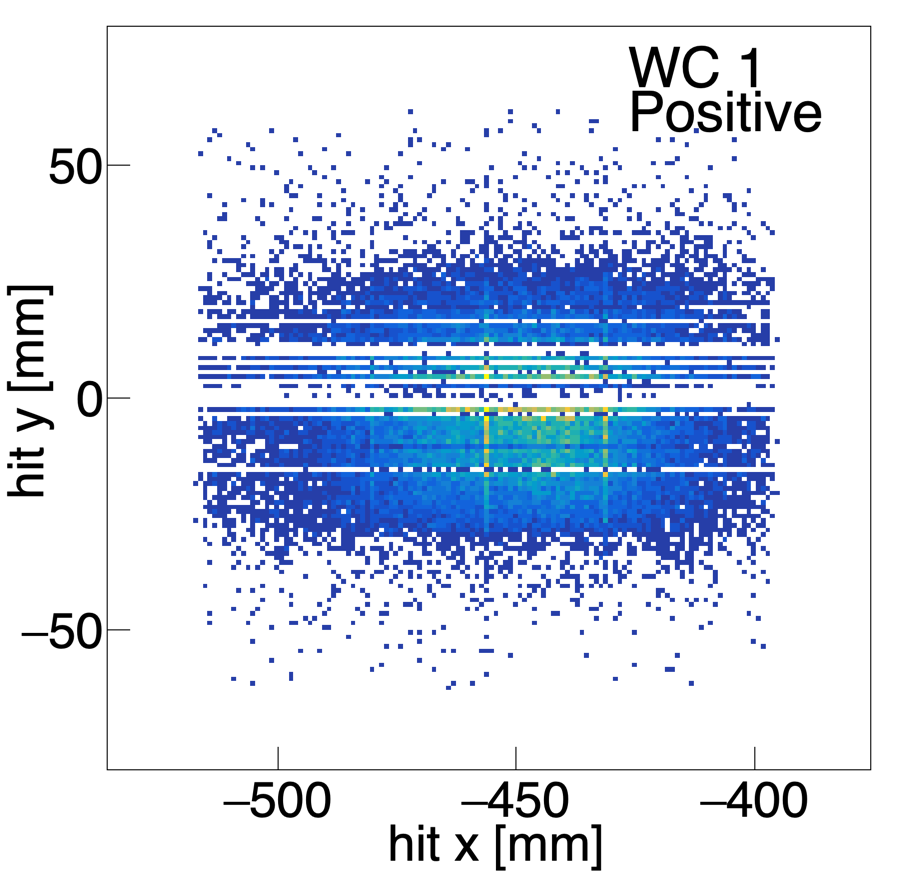
\includegraphics[width=\textwidth]{wcn_xy1_pol1_period4.png}
            \caption{WC1, P4}
            \label{fig_wc1_p4}
            \end{subfigure}
            \hfill             
             \begin{subfigure}[b]{0.23\textwidth}
            \centering
            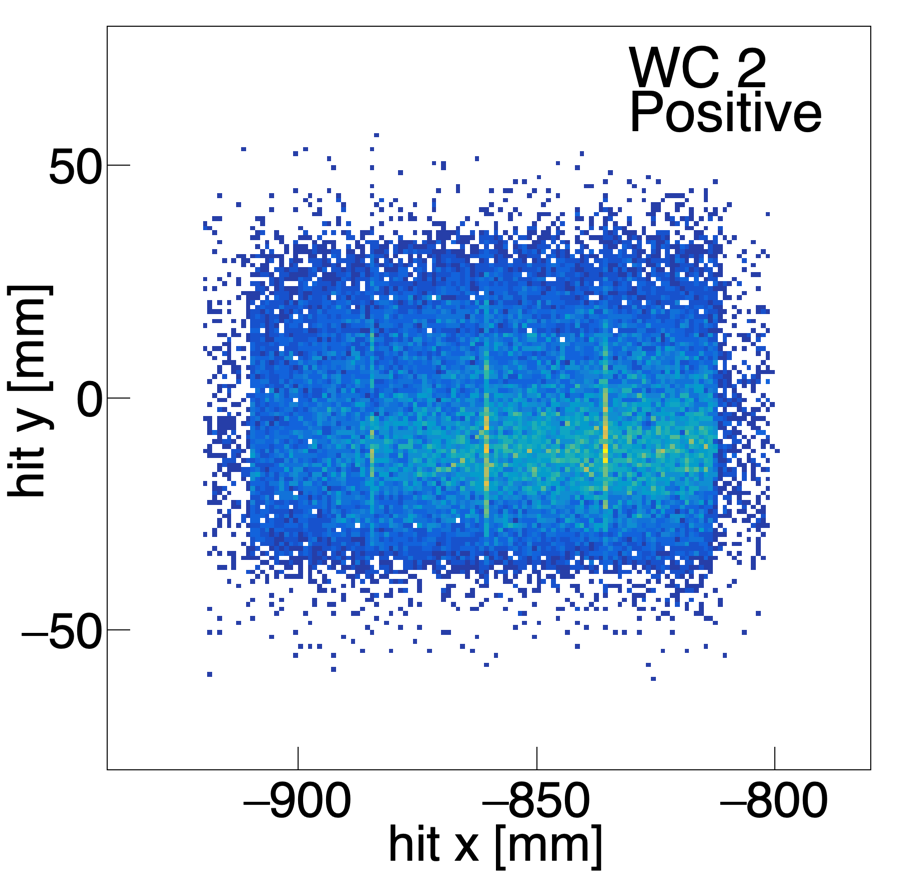
\includegraphics[width=\textwidth]{wcn_xy2_pol1_period4.png}
            \caption{WC2, P4}
            \label{fig_wc2_p4}
            \end{subfigure}
            \hfill 
              \begin{subfigure}[b]{0.23\textwidth}
            \centering
            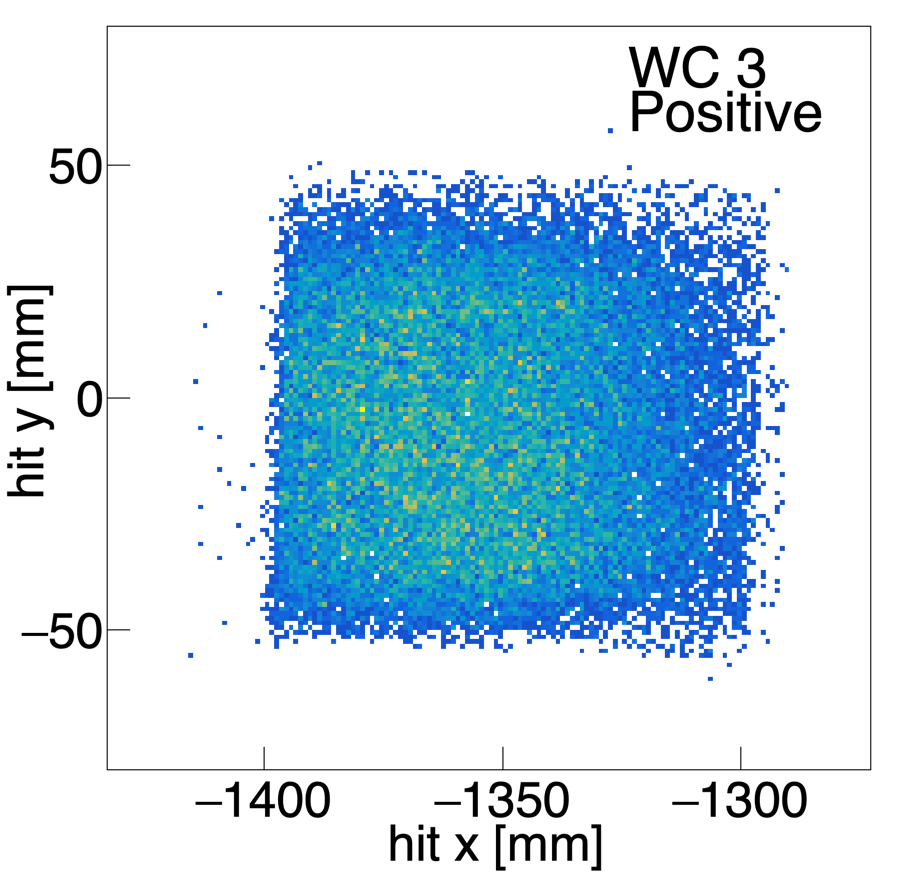
\includegraphics[width=\textwidth]{wcn_xy3_pol1_period4.png}
            \caption{WC3, P4}
            \label{fig_wc3_p4}
            \end{subfigure}
            \hfill    
             \begin{subfigure}[b]{0.23\textwidth}
            \centering
            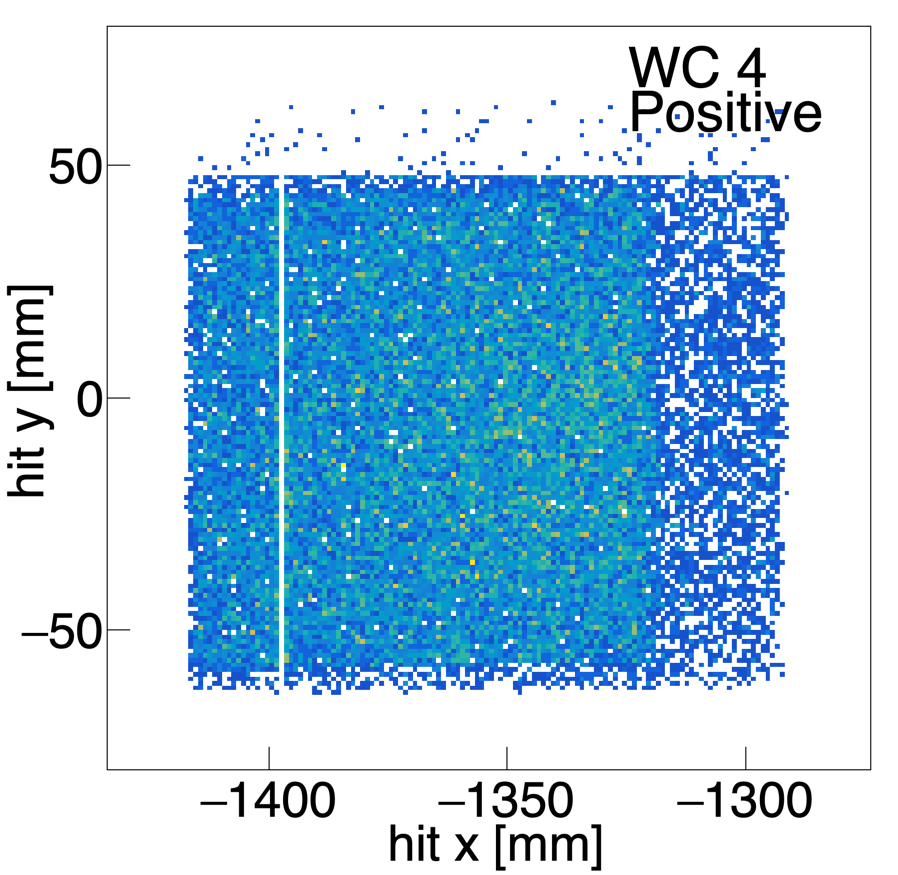
\includegraphics[width=\textwidth]{wcn_xy4_pol1_period4.png}
            \caption{WC4, P4}
            \label{fig_wc4_p4}
            \end{subfigure}
            \hfill
   \caption[short]{The WCTrack best hit position in each of the four wire chambers, in period 4, divided by polarity.}
   \label{fig_xyhitspol}
  \end{figure}
  
  
  
\newpage

\subsection{The rotation of the magnet}

Figure~\ref{fig_magnet} shows a sketch of a track passing through the magnetic field. The magnet is rotated about its center, contrary to what is shown in the technical drawings Figures~\ref{fig_td1} and ~\ref{fig_td2} . Figure~\ref{fig_xymag} show the entry point in x,y in the magnet's frame of the upstream track. 

\begin{figure}[h]	   
 \centering
        	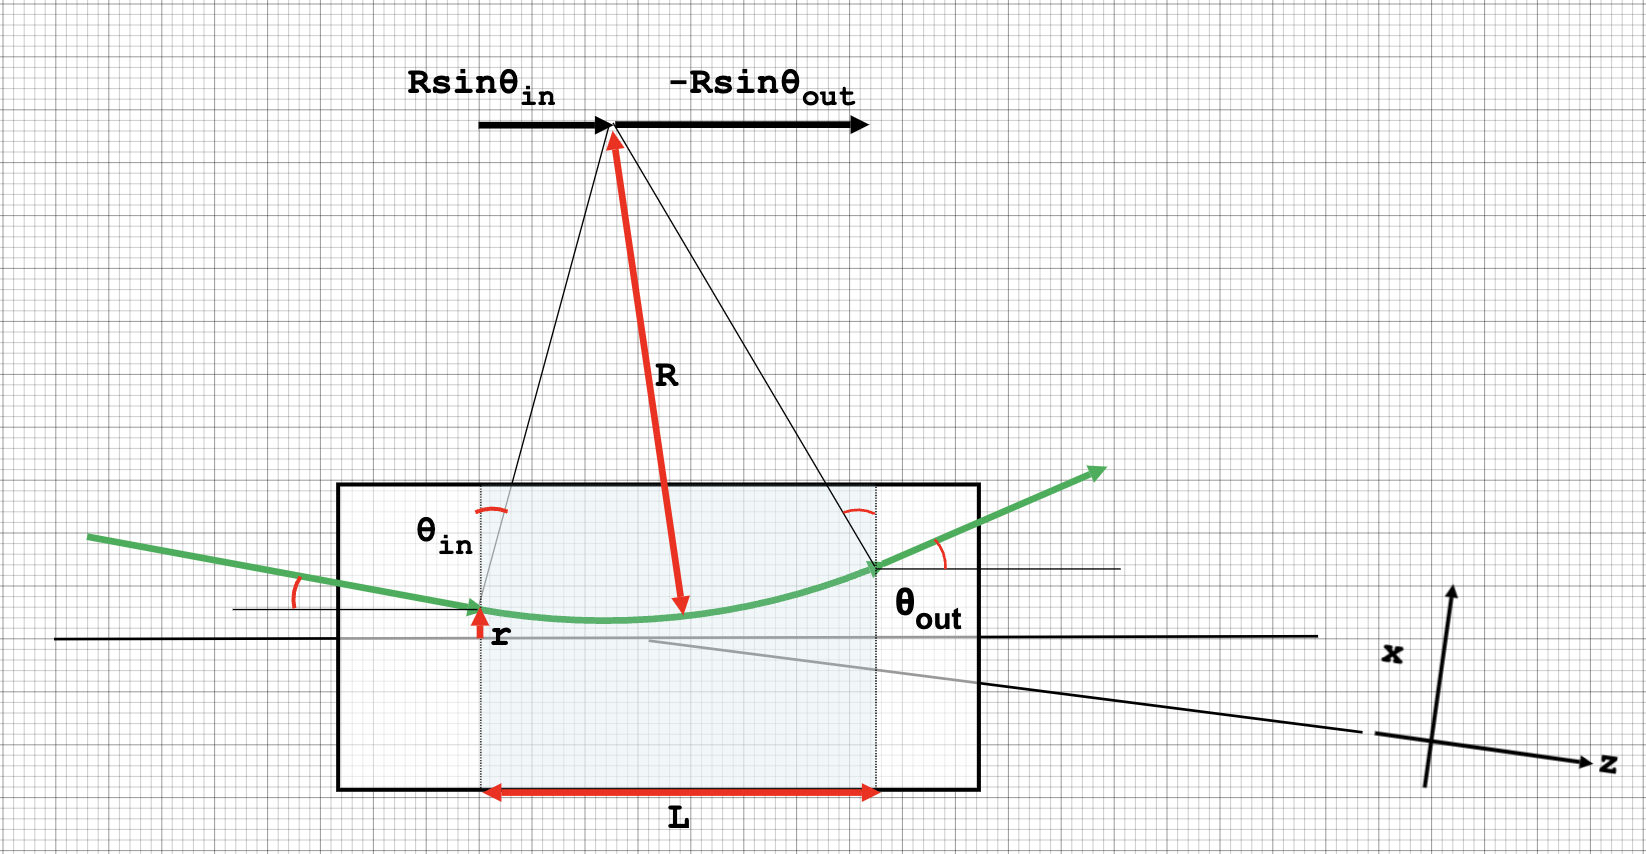
\includegraphics[scale=0.5]{magnet-detail.png}	 
   \caption[short]{Magnet details.}
   \label{fig_magnet}
  \end{figure}
  
  \begin{figure}[h]	   
 \centering
        	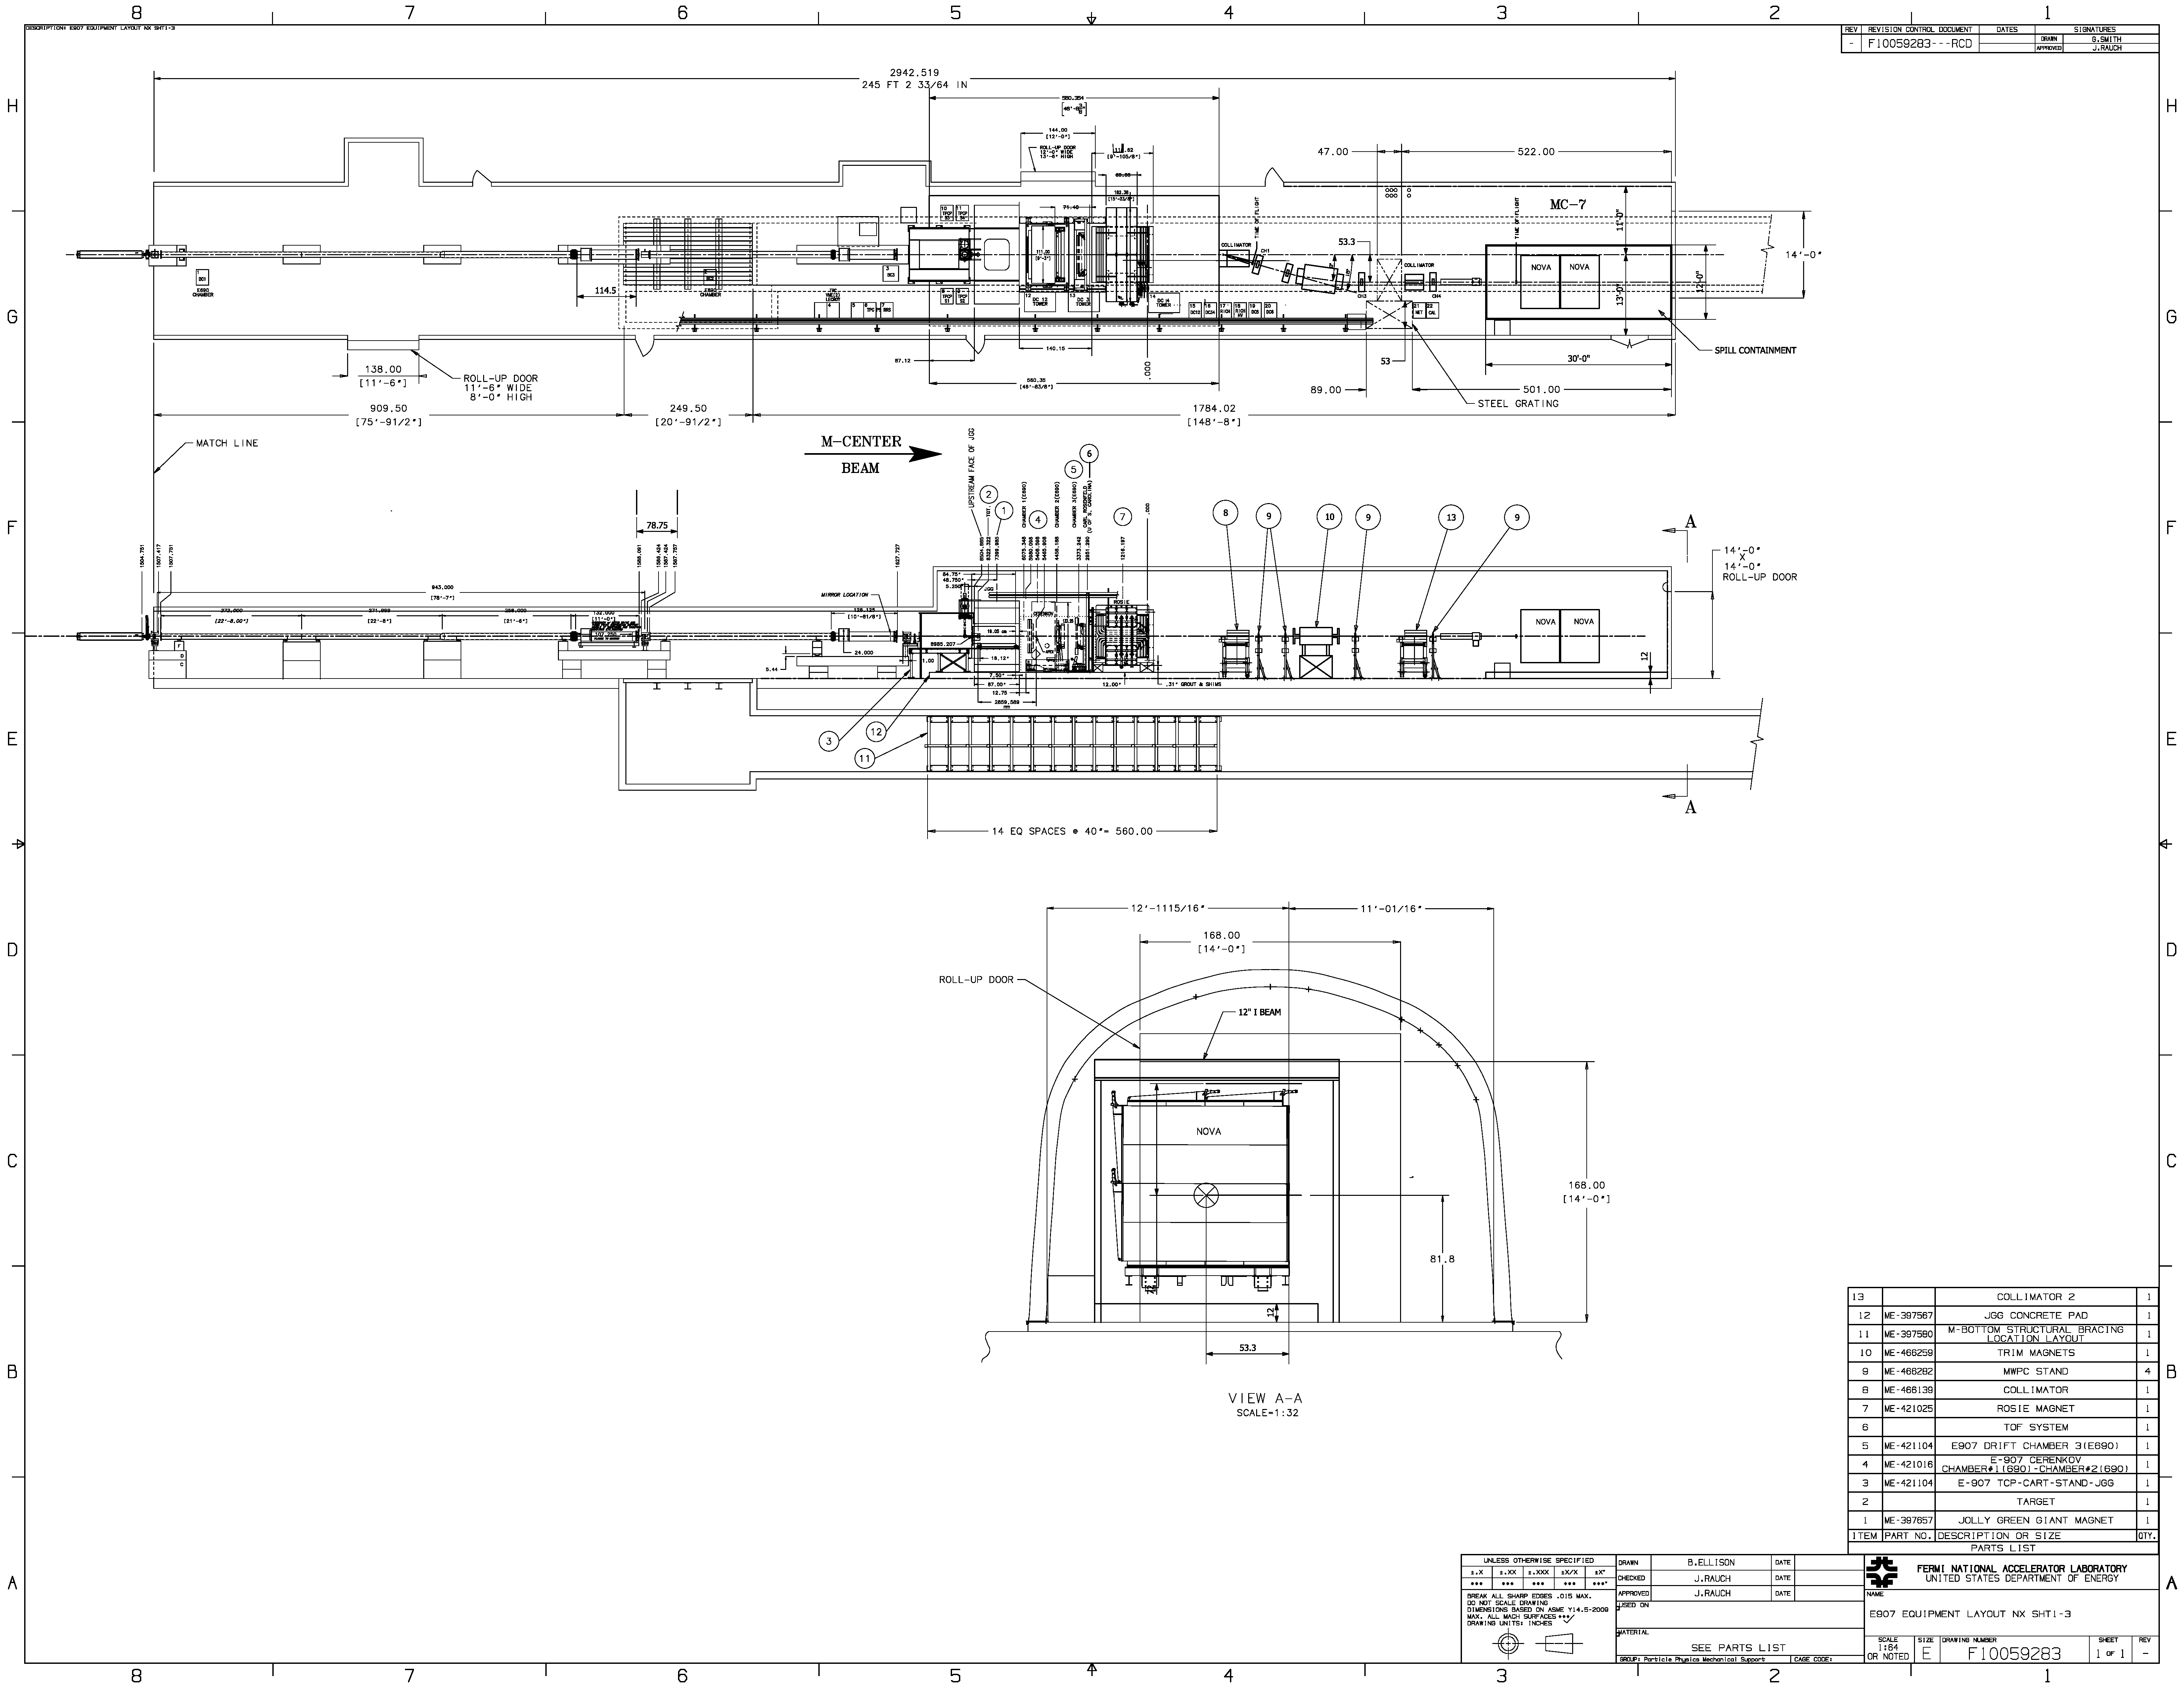
\includegraphics[scale=0.5]{ftbf_drawing.april_2018.pdf}	 
   \caption[short]{Technical drawing made before the decision to rotate the magnet around its center rather than its front face center.}
   \label{fig_td1}
  \end{figure}
  
    \begin{figure}[h]	   
 \centering
        	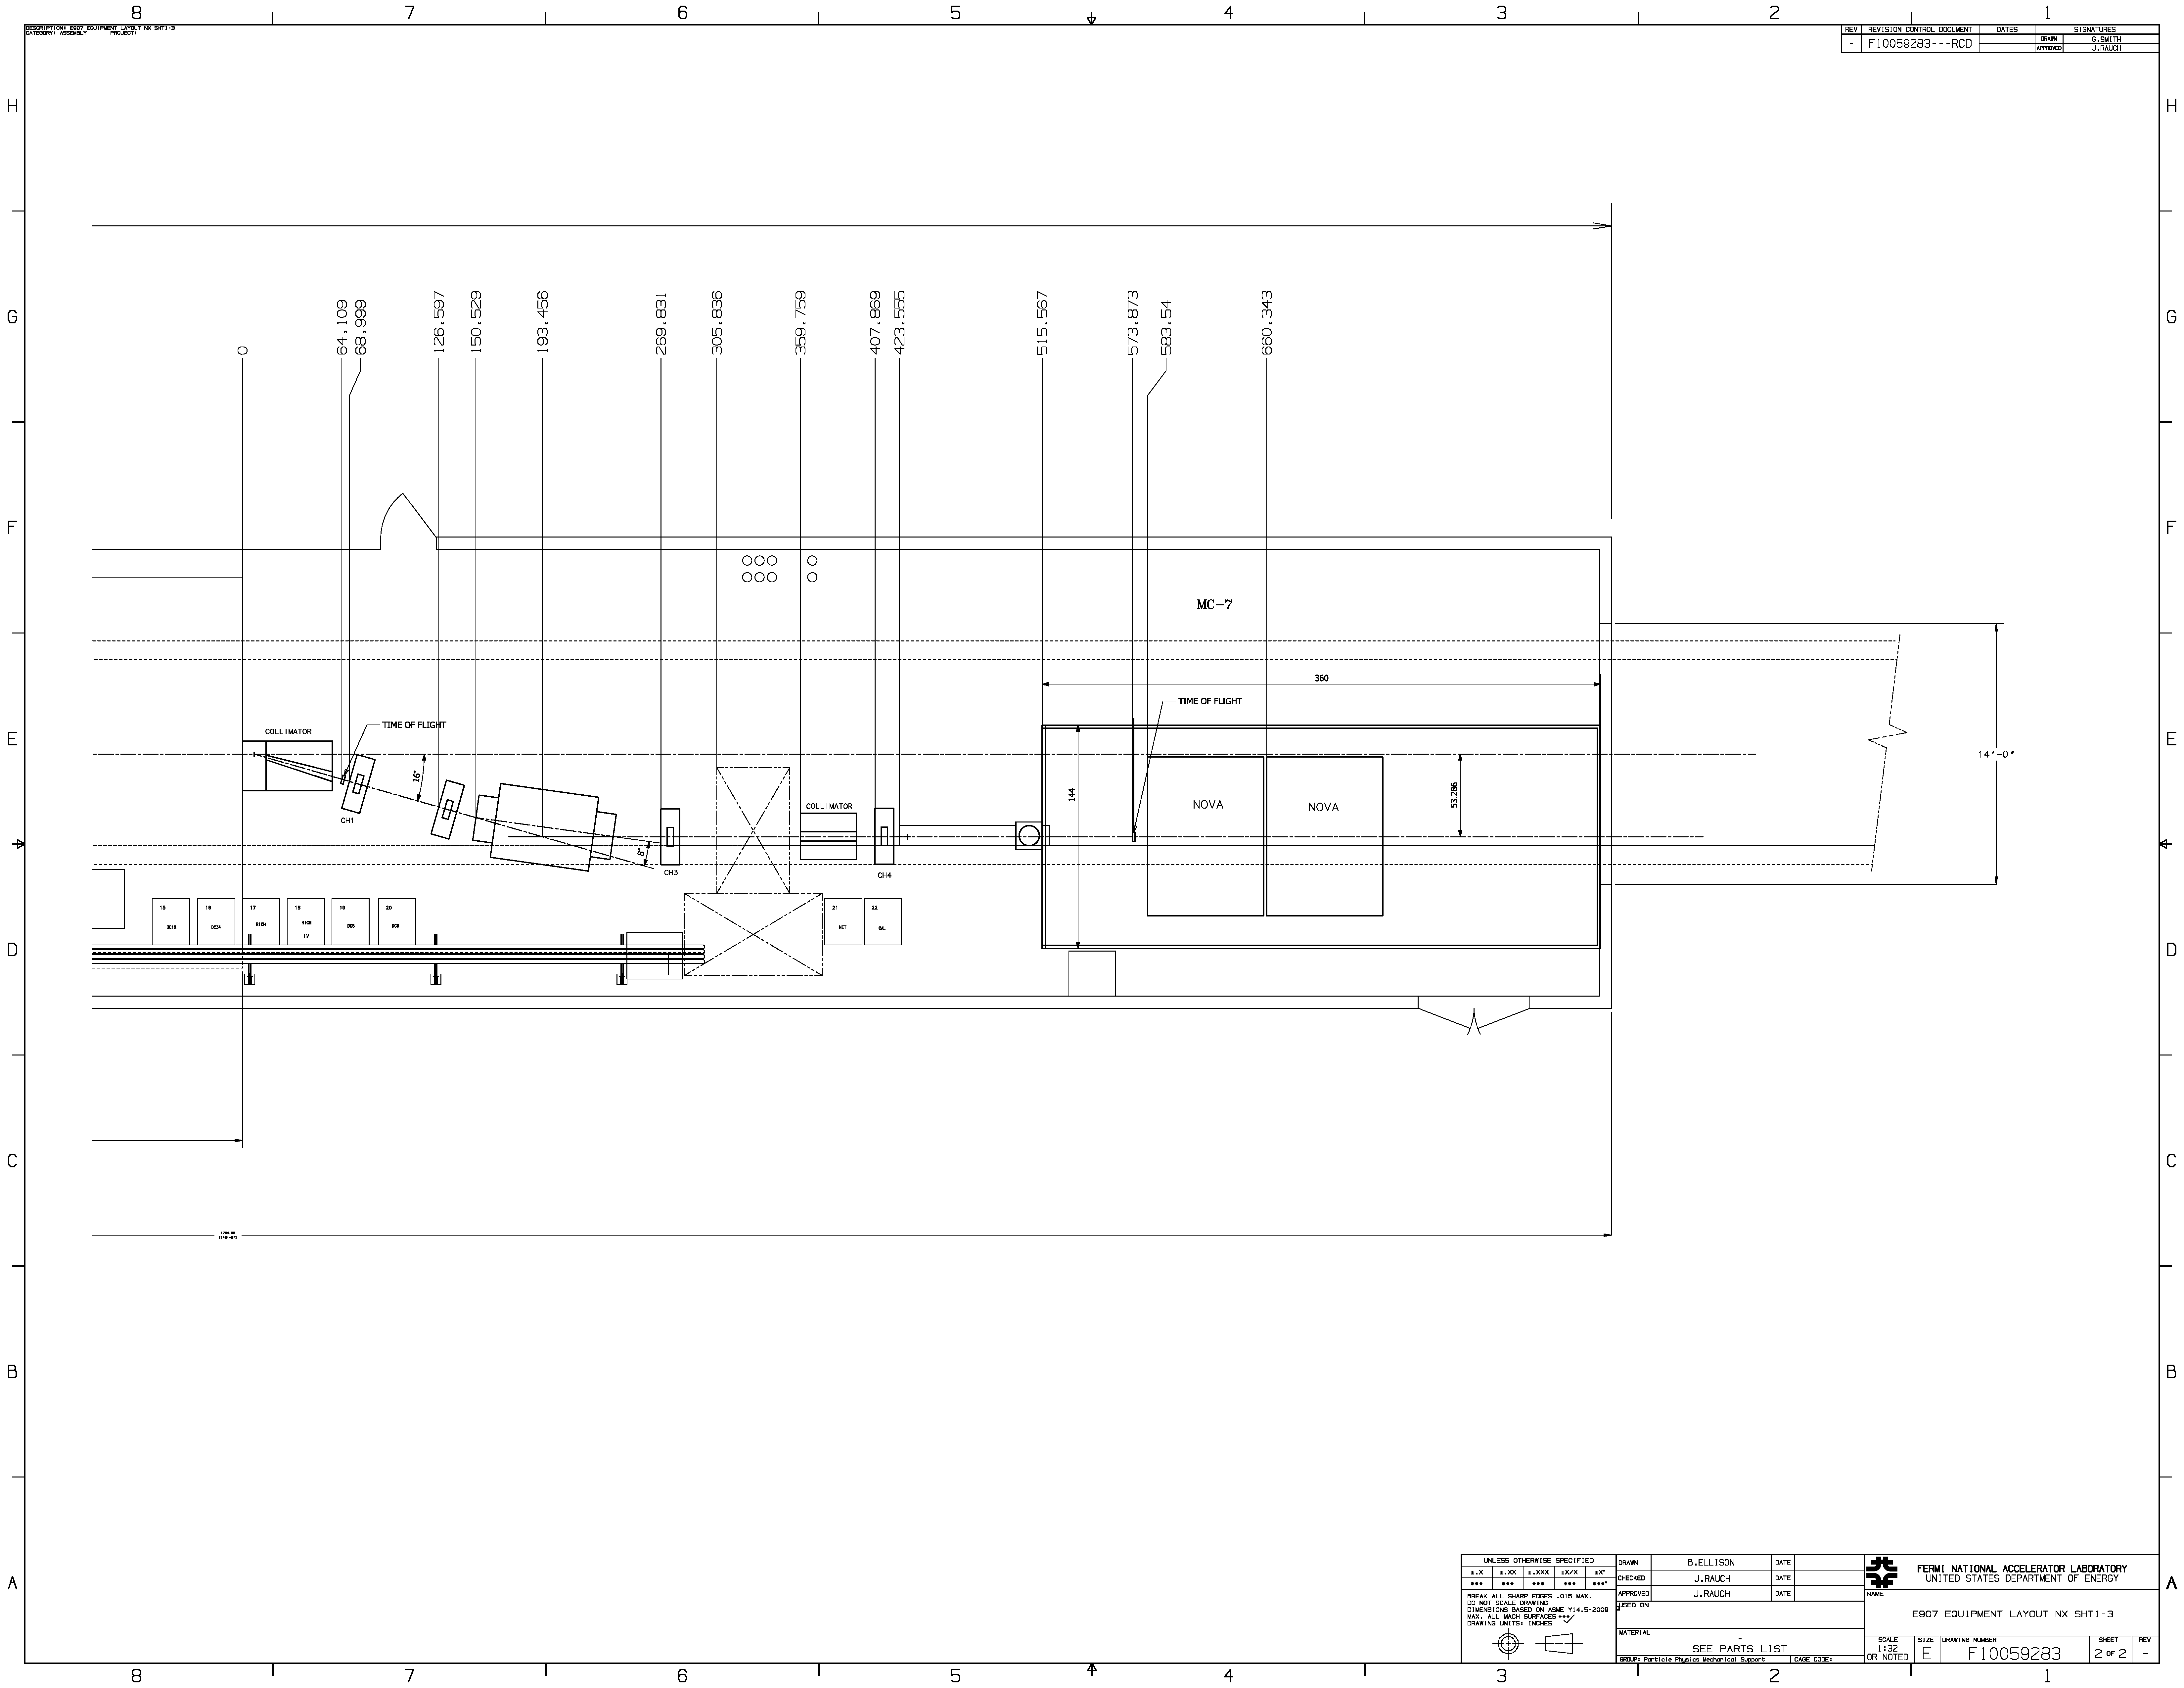
\includegraphics[scale=0.5]{gsmith_F10059283.may_2018.pdf}	 
   \caption[short]{Technical drawing made before the decision to rotate the magnet around its center rather than its front face center.}
   \label{fig_td2}
  \end{figure}
  
  

       \begin{figure}[h]	   
            \centering
%   
%            \begin{subfigure}[b]{0.48\textwidth}
%            \centering
            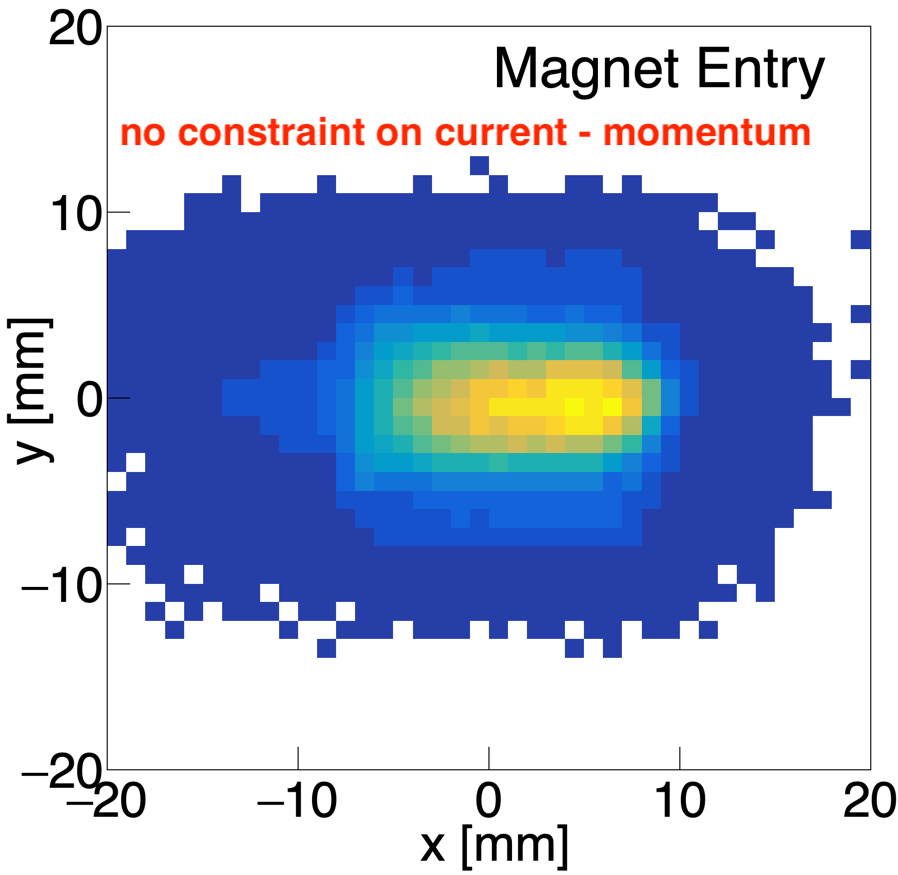
\includegraphics[scale=0.3]{wcn_mexy_pol-1_period234.png}
%            \caption{$y=x$}
%            \label{fig:y equals x}
%            \end{subfigure}
%            \hfill             
%             \begin{subfigure}[b]{0.48\textwidth}
%            \centering
%            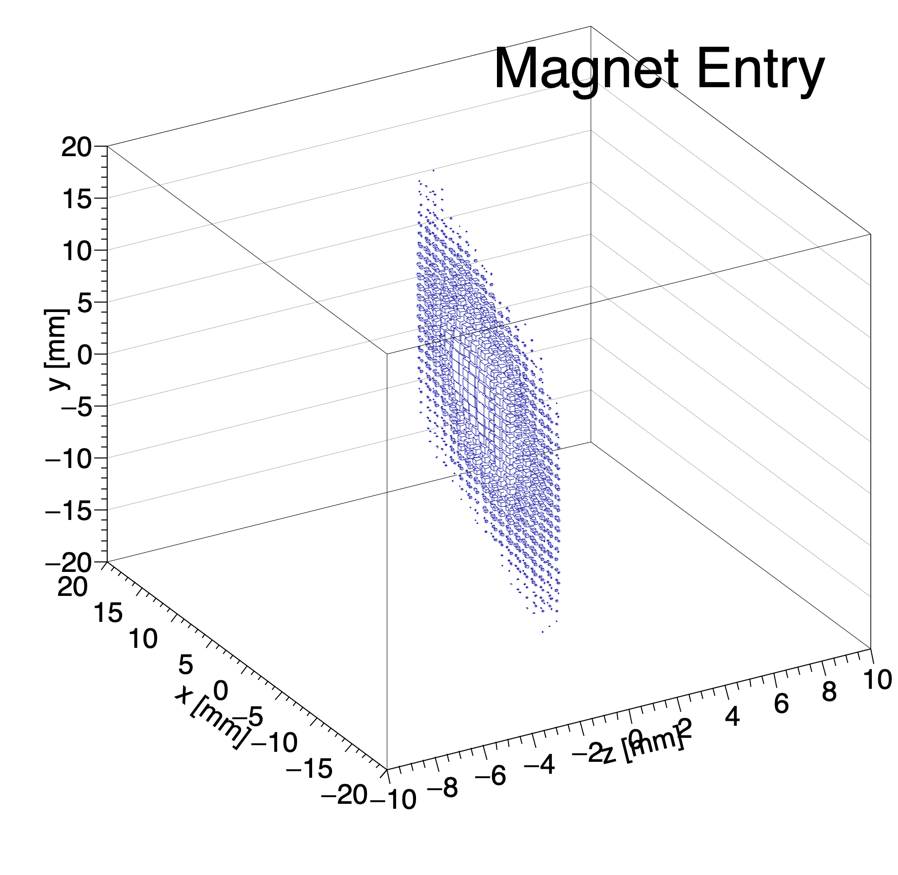
\includegraphics[width=\textwidth]{wcn_mexyz_pol-1_period234.png}
%            \caption{$y=x$}
%            \label{fig:y equals x}
%            \end{subfigure}
   \caption[short]{The x,y entry point of the upstream track to the magnetic field.}
   \label{fig_xymag}
  \end{figure}
  

  
  
  

\subsection{The baby NOvA coordinates}


Figure~\ref{fig_novarot} shows the  detector rotation.

\begin{figure}[h]	   
 \centering
        	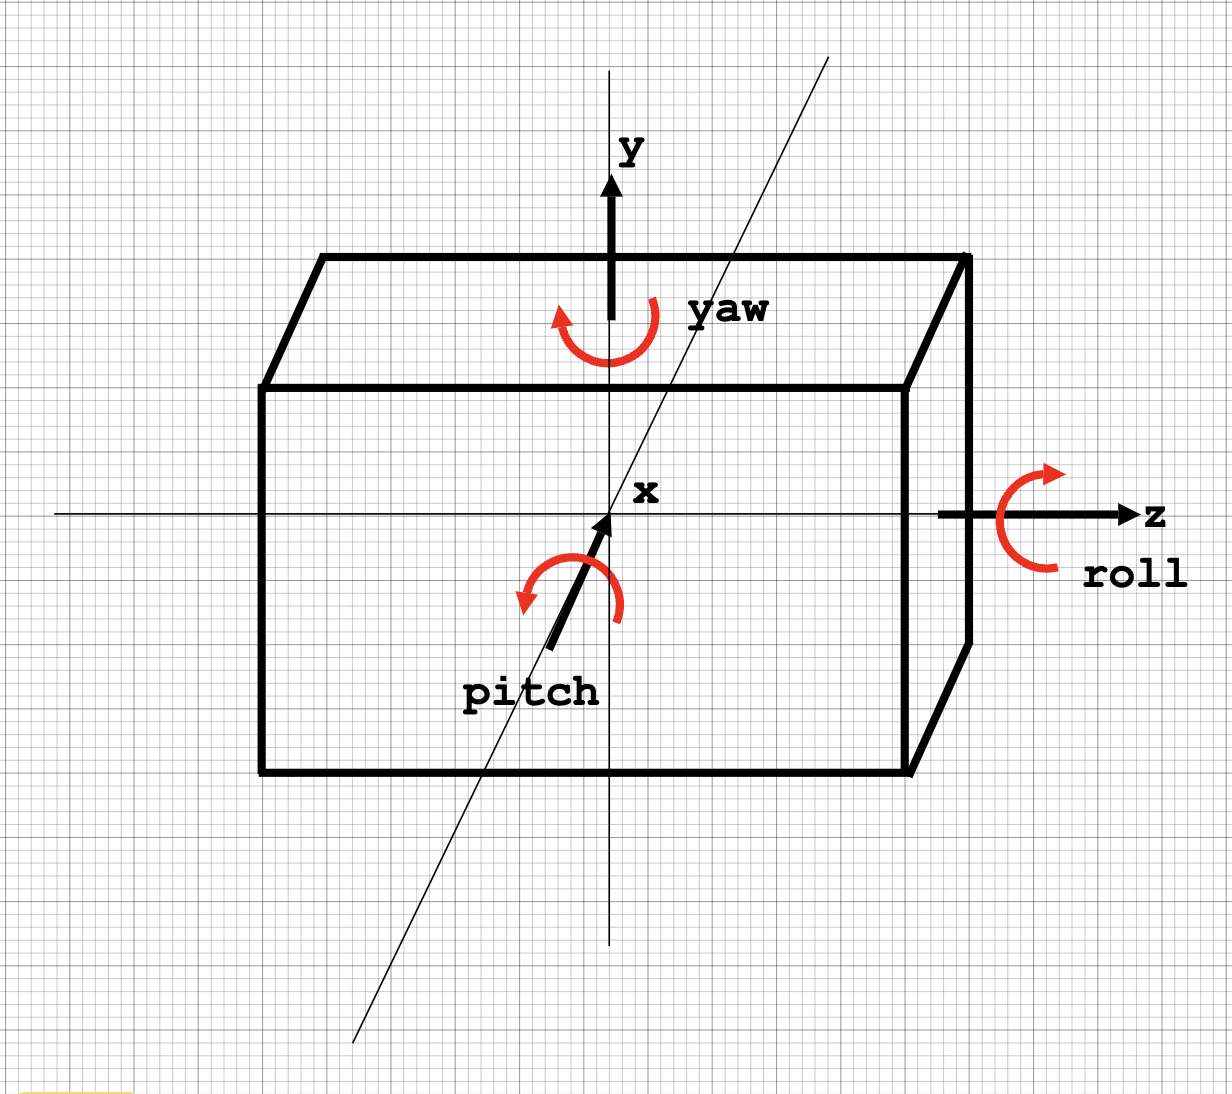
\includegraphics[scale=0.5]{novarot.png}	 
   \caption[short]{NOvA rotation.}
   \label{fig_novarot}
  \end{figure}
 
